\documentclass[conference]{IEEEtran}
\usepackage[T1]{fontenc}
\usepackage{graphicx}
\usepackage{booktabs}
\usepackage{amsmath}
\usepackage{cite}
\usepackage{url}
\usepackage{xspace}
\usepackage{placeins}
\usepackage{stfloats}
\fnbelowfloat

\newcommand{\papertitle}{PlaceIQ: Explainable Semantic Shortlisting for Campus Placement}
% Generated by eval/make_paper_numbers.py from eval/results/*. Do not edit by hand.
\newcommand{\NStudents}{500}
\newcommand{\NRequirements}{15}
\newcommand{\NDev}{5}
\newcommand{\NTest}{10}
\newcommand{\NQualifiedDev}{114}
\newcommand{\NQualifiedTest}{190}
\newcommand{\NQualifiedTestMin}{14}
\newcommand{\NQualifiedTestMax}{29}
\newcommand{\NPairs}{7500}
\newcommand{\NArchParaphrased}{100}
\newcommand{\NArchSparseStrong}{40}
\newcommand{\NArchStandard}{150}
\newcommand{\NArchAbbreviatedNoisy}{50}
\newcommand{\NArchStuffedWeak}{50}
\newcommand{\NArchGeneralistAverage}{25}
\newcommand{\NArchImplied}{50}
\newcommand{\NArchIneligibleStrong}{35}
\newcommand{\NSkills}{71}
\newcommand{\AtsStrictNdcgMean}{0.479}
\newcommand{\AtsStrictNdcgLo}{0.307}
\newcommand{\AtsStrictNdcgHi}{0.633}
\newcommand{\AtsStrictNdcgCi}{0.479 [0.307, 0.633]}
\newcommand{\AtsStrictMrrMean}{0.650}
\newcommand{\AtsStrictMrrLo}{0.400}
\newcommand{\AtsStrictMrrHi}{0.900}
\newcommand{\AtsStrictMrrCi}{0.650 [0.400, 0.900]}
\newcommand{\AtsStrictPtenMean}{0.590}
\newcommand{\AtsStrictPtenLo}{0.370}
\newcommand{\AtsStrictPtenHi}{0.790}
\newcommand{\AtsStrictPtenCi}{0.590 [0.370, 0.790]}
\newcommand{\AtsStrictRplainMean}{0.311}
\newcommand{\AtsStrictRplainLo}{0.196}
\newcommand{\AtsStrictRplainHi}{0.417}
\newcommand{\AtsStrictRplainCi}{0.311 [0.196, 0.417]}
\newcommand{\AtsStrictRcapMean}{0.590}
\newcommand{\AtsStrictRcapLo}{0.370}
\newcommand{\AtsStrictRcapHi}{0.790}
\newcommand{\AtsStrictRcapCi}{0.590 [0.370, 0.790]}
\newcommand{\AtsStrictFrrtenMean}{0.410}
\newcommand{\AtsStrictFrrtenLo}{0.210}
\newcommand{\AtsStrictFrrtenHi}{0.630}
\newcommand{\AtsStrictFrrtenCi}{0.410 [0.210, 0.630]}
\newcommand{\AtsStrictFrrtwentyMean}{0.529}
\newcommand{\AtsStrictFrrtwentyLo}{0.340}
\newcommand{\AtsStrictFrrtwentyHi}{0.716}
\newcommand{\AtsStrictFrrtwentyCi}{0.529 [0.340, 0.716]}
\newcommand{\AtsLenientNdcgMean}{0.607}
\newcommand{\AtsLenientNdcgLo}{0.501}
\newcommand{\AtsLenientNdcgHi}{0.707}
\newcommand{\AtsLenientNdcgCi}{0.607 [0.501, 0.707]}
\newcommand{\AtsLenientMrrMean}{0.783}
\newcommand{\AtsLenientMrrLo}{0.617}
\newcommand{\AtsLenientMrrHi}{0.950}
\newcommand{\AtsLenientMrrCi}{0.783 [0.617, 0.950]}
\newcommand{\AtsLenientPtenMean}{0.700}
\newcommand{\AtsLenientPtenLo}{0.640}
\newcommand{\AtsLenientPtenHi}{0.750}
\newcommand{\AtsLenientPtenCi}{0.700 [0.640, 0.750]}
\newcommand{\AtsLenientRplainMean}{0.386}
\newcommand{\AtsLenientRplainLo}{0.327}
\newcommand{\AtsLenientRplainHi}{0.449}
\newcommand{\AtsLenientRplainCi}{0.386 [0.327, 0.449]}
\newcommand{\AtsLenientRcapMean}{0.700}
\newcommand{\AtsLenientRcapLo}{0.640}
\newcommand{\AtsLenientRcapHi}{0.750}
\newcommand{\AtsLenientRcapCi}{0.700 [0.640, 0.750]}
\newcommand{\AtsLenientFrrtenMean}{0.300}
\newcommand{\AtsLenientFrrtenLo}{0.250}
\newcommand{\AtsLenientFrrtenHi}{0.360}
\newcommand{\AtsLenientFrrtenCi}{0.300 [0.250, 0.360]}
\newcommand{\AtsLenientFrrtwentyMean}{0.397}
\newcommand{\AtsLenientFrrtwentyLo}{0.336}
\newcommand{\AtsLenientFrrtwentyHi}{0.456}
\newcommand{\AtsLenientFrrtwentyCi}{0.397 [0.336, 0.456]}
\newcommand{\AtsSynNdcgMean}{0.639}
\newcommand{\AtsSynNdcgLo}{0.564}
\newcommand{\AtsSynNdcgHi}{0.711}
\newcommand{\AtsSynNdcgCi}{0.639 [0.564, 0.711]}
\newcommand{\AtsSynMrrMean}{0.850}
\newcommand{\AtsSynMrrLo}{0.700}
\newcommand{\AtsSynMrrHi}{1.000}
\newcommand{\AtsSynMrrCi}{0.850 [0.700, 1.000]}
\newcommand{\AtsSynPtenMean}{0.730}
\newcommand{\AtsSynPtenLo}{0.610}
\newcommand{\AtsSynPtenHi}{0.830}
\newcommand{\AtsSynPtenCi}{0.730 [0.610, 0.830]}
\newcommand{\AtsSynRplainMean}{0.389}
\newcommand{\AtsSynRplainLo}{0.334}
\newcommand{\AtsSynRplainHi}{0.447}
\newcommand{\AtsSynRplainCi}{0.389 [0.334, 0.447]}
\newcommand{\AtsSynRcapMean}{0.730}
\newcommand{\AtsSynRcapLo}{0.610}
\newcommand{\AtsSynRcapHi}{0.830}
\newcommand{\AtsSynRcapCi}{0.730 [0.610, 0.830]}
\newcommand{\AtsSynFrrtenMean}{0.270}
\newcommand{\AtsSynFrrtenLo}{0.170}
\newcommand{\AtsSynFrrtenHi}{0.390}
\newcommand{\AtsSynFrrtenCi}{0.270 [0.170, 0.390]}
\newcommand{\AtsSynFrrtwentyMean}{0.338}
\newcommand{\AtsSynFrrtwentyLo}{0.233}
\newcommand{\AtsSynFrrtwentyHi}{0.462}
\newcommand{\AtsSynFrrtwentyCi}{0.338 [0.233, 0.462]}
\newcommand{\BmNdcgMean}{0.685}
\newcommand{\BmNdcgLo}{0.597}
\newcommand{\BmNdcgHi}{0.774}
\newcommand{\BmNdcgCi}{0.685 [0.597, 0.774]}
\newcommand{\BmMrrMean}{0.900}
\newcommand{\BmMrrLo}{0.750}
\newcommand{\BmMrrHi}{1.000}
\newcommand{\BmMrrCi}{0.900 [0.750, 1.000]}
\newcommand{\BmPtenMean}{0.790}
\newcommand{\BmPtenLo}{0.670}
\newcommand{\BmPtenHi}{0.890}
\newcommand{\BmPtenCi}{0.790 [0.670, 0.890]}
\newcommand{\BmRplainMean}{0.428}
\newcommand{\BmRplainLo}{0.361}
\newcommand{\BmRplainHi}{0.507}
\newcommand{\BmRplainCi}{0.428 [0.361, 0.507]}
\newcommand{\BmRcapMean}{0.790}
\newcommand{\BmRcapLo}{0.670}
\newcommand{\BmRcapHi}{0.890}
\newcommand{\BmRcapCi}{0.790 [0.670, 0.890]}
\newcommand{\BmFrrtenMean}{0.210}
\newcommand{\BmFrrtenLo}{0.110}
\newcommand{\BmFrrtenHi}{0.330}
\newcommand{\BmFrrtenCi}{0.210 [0.110, 0.330]}
\newcommand{\BmFrrtwentyMean}{0.329}
\newcommand{\BmFrrtwentyLo}{0.244}
\newcommand{\BmFrrtwentyHi}{0.410}
\newcommand{\BmFrrtwentyCi}{0.329 [0.244, 0.410]}
\newcommand{\DenseNdcgMean}{0.636}
\newcommand{\DenseNdcgLo}{0.530}
\newcommand{\DenseNdcgHi}{0.733}
\newcommand{\DenseNdcgCi}{0.636 [0.530, 0.733]}
\newcommand{\DenseMrrMean}{0.950}
\newcommand{\DenseMrrLo}{0.850}
\newcommand{\DenseMrrHi}{1.000}
\newcommand{\DenseMrrCi}{0.950 [0.850, 1.000]}
\newcommand{\DensePtenMean}{0.620}
\newcommand{\DensePtenLo}{0.490}
\newcommand{\DensePtenHi}{0.750}
\newcommand{\DensePtenCi}{0.620 [0.490, 0.750]}
\newcommand{\DenseRplainMean}{0.322}
\newcommand{\DenseRplainLo}{0.276}
\newcommand{\DenseRplainHi}{0.359}
\newcommand{\DenseRplainCi}{0.322 [0.276, 0.359]}
\newcommand{\DenseRcapMean}{0.620}
\newcommand{\DenseRcapLo}{0.490}
\newcommand{\DenseRcapHi}{0.750}
\newcommand{\DenseRcapCi}{0.620 [0.490, 0.750]}
\newcommand{\DenseFrrtenMean}{0.380}
\newcommand{\DenseFrrtenLo}{0.250}
\newcommand{\DenseFrrtenHi}{0.510}
\newcommand{\DenseFrrtenCi}{0.380 [0.250, 0.510]}
\newcommand{\DenseFrrtwentyMean}{0.501}
\newcommand{\DenseFrrtwentyLo}{0.440}
\newcommand{\DenseFrrtwentyHi}{0.560}
\newcommand{\DenseFrrtwentyCi}{0.501 [0.440, 0.560]}
\newcommand{\HybridNdcgMean}{0.718}
\newcommand{\HybridNdcgLo}{0.633}
\newcommand{\HybridNdcgHi}{0.794}
\newcommand{\HybridNdcgCi}{0.718 [0.633, 0.794]}
\newcommand{\HybridMrrMean}{0.900}
\newcommand{\HybridMrrLo}{0.750}
\newcommand{\HybridMrrHi}{1.000}
\newcommand{\HybridMrrCi}{0.900 [0.750, 1.000]}
\newcommand{\HybridPtenMean}{0.800}
\newcommand{\HybridPtenLo}{0.710}
\newcommand{\HybridPtenHi}{0.890}
\newcommand{\HybridPtenCi}{0.800 [0.710, 0.890]}
\newcommand{\HybridRplainMean}{0.428}
\newcommand{\HybridRplainLo}{0.393}
\newcommand{\HybridRplainHi}{0.465}
\newcommand{\HybridRplainCi}{0.428 [0.393, 0.465]}
\newcommand{\HybridRcapMean}{0.800}
\newcommand{\HybridRcapLo}{0.710}
\newcommand{\HybridRcapHi}{0.890}
\newcommand{\HybridRcapCi}{0.800 [0.710, 0.890]}
\newcommand{\HybridFrrtenMean}{0.200}
\newcommand{\HybridFrrtenLo}{0.110}
\newcommand{\HybridFrrtenHi}{0.290}
\newcommand{\HybridFrrtenCi}{0.200 [0.110, 0.290]}
\newcommand{\HybridFrrtwentyMean}{0.314}
\newcommand{\HybridFrrtwentyLo}{0.233}
\newcommand{\HybridFrrtwentyHi}{0.384}
\newcommand{\HybridFrrtwentyCi}{0.314 [0.233, 0.384]}
\newcommand{\PropNdcgMean}{0.749}
\newcommand{\PropNdcgLo}{0.674}
\newcommand{\PropNdcgHi}{0.818}
\newcommand{\PropNdcgCi}{0.749 [0.674, 0.818]}
\newcommand{\PropMrrMean}{1.000}
\newcommand{\PropMrrLo}{1.000}
\newcommand{\PropMrrHi}{1.000}
\newcommand{\PropMrrCi}{1.000 [1.000, 1.000]}
\newcommand{\PropPtenMean}{0.760}
\newcommand{\PropPtenLo}{0.630}
\newcommand{\PropPtenHi}{0.870}
\newcommand{\PropPtenCi}{0.760 [0.630, 0.870]}
\newcommand{\PropRplainMean}{0.403}
\newcommand{\PropRplainLo}{0.344}
\newcommand{\PropRplainHi}{0.449}
\newcommand{\PropRplainCi}{0.403 [0.344, 0.449]}
\newcommand{\PropRcapMean}{0.760}
\newcommand{\PropRcapLo}{0.630}
\newcommand{\PropRcapHi}{0.870}
\newcommand{\PropRcapCi}{0.760 [0.630, 0.870]}
\newcommand{\PropFrrtenMean}{0.240}
\newcommand{\PropFrrtenLo}{0.130}
\newcommand{\PropFrrtenHi}{0.370}
\newcommand{\PropFrrtenCi}{0.240 [0.130, 0.370]}
\newcommand{\PropFrrtwentyMean}{0.501}
\newcommand{\PropFrrtwentyLo}{0.440}
\newcommand{\PropFrrtwentyHi}{0.560}
\newcommand{\PropFrrtwentyCi}{0.501 [0.440, 0.560]}
\newcommand{\PropKfiftyNdcgMean}{0.763}
\newcommand{\PropKfiftyNdcgLo}{0.694}
\newcommand{\PropKfiftyNdcgHi}{0.824}
\newcommand{\PropKfiftyNdcgCi}{0.763 [0.694, 0.824]}
\newcommand{\PropKfiftyMrrMean}{1.000}
\newcommand{\PropKfiftyMrrLo}{1.000}
\newcommand{\PropKfiftyMrrHi}{1.000}
\newcommand{\PropKfiftyMrrCi}{1.000 [1.000, 1.000]}
\newcommand{\PropKfiftyPtenMean}{0.770}
\newcommand{\PropKfiftyPtenLo}{0.640}
\newcommand{\PropKfiftyPtenHi}{0.860}
\newcommand{\PropKfiftyPtenCi}{0.770 [0.640, 0.860]}
\newcommand{\PropKfiftyRplainMean}{0.411}
\newcommand{\PropKfiftyRplainLo}{0.351}
\newcommand{\PropKfiftyRplainHi}{0.458}
\newcommand{\PropKfiftyRplainCi}{0.411 [0.351, 0.458]}
\newcommand{\PropKfiftyRcapMean}{0.770}
\newcommand{\PropKfiftyRcapLo}{0.640}
\newcommand{\PropKfiftyRcapHi}{0.860}
\newcommand{\PropKfiftyRcapCi}{0.770 [0.640, 0.860]}
\newcommand{\PropKfiftyFrrtenMean}{0.230}
\newcommand{\PropKfiftyFrrtenLo}{0.140}
\newcommand{\PropKfiftyFrrtenHi}{0.360}
\newcommand{\PropKfiftyFrrtenCi}{0.230 [0.140, 0.360]}
\newcommand{\PropKfiftyFrrtwentyMean}{0.308}
\newcommand{\PropKfiftyFrrtwentyLo}{0.237}
\newcommand{\PropKfiftyFrrtwentyHi}{0.376}
\newcommand{\PropKfiftyFrrtwentyCi}{0.308 [0.237, 0.376]}
\newcommand{\PropOracleNdcgMean}{0.755}
\newcommand{\PropOracleNdcgLo}{0.679}
\newcommand{\PropOracleNdcgHi}{0.824}
\newcommand{\PropOracleNdcgCi}{0.755 [0.679, 0.824]}
\newcommand{\PropOracleMrrMean}{1.000}
\newcommand{\PropOracleMrrLo}{1.000}
\newcommand{\PropOracleMrrHi}{1.000}
\newcommand{\PropOracleMrrCi}{1.000 [1.000, 1.000]}
\newcommand{\PropOraclePtenMean}{0.770}
\newcommand{\PropOraclePtenLo}{0.640}
\newcommand{\PropOraclePtenHi}{0.880}
\newcommand{\PropOraclePtenCi}{0.770 [0.640, 0.880]}
\newcommand{\PropOracleRplainMean}{0.409}
\newcommand{\PropOracleRplainLo}{0.346}
\newcommand{\PropOracleRplainHi}{0.458}
\newcommand{\PropOracleRplainCi}{0.409 [0.346, 0.458]}
\newcommand{\PropOracleRcapMean}{0.770}
\newcommand{\PropOracleRcapLo}{0.640}
\newcommand{\PropOracleRcapHi}{0.880}
\newcommand{\PropOracleRcapCi}{0.770 [0.640, 0.880]}
\newcommand{\PropOracleFrrtenMean}{0.230}
\newcommand{\PropOracleFrrtenLo}{0.120}
\newcommand{\PropOracleFrrtenHi}{0.360}
\newcommand{\PropOracleFrrtenCi}{0.230 [0.120, 0.360]}
\newcommand{\PropOracleFrrtwentyMean}{0.495}
\newcommand{\PropOracleFrrtwentyLo}{0.437}
\newcommand{\PropOracleFrrtwentyHi}{0.554}
\newcommand{\PropOracleFrrtwentyCi}{0.495 [0.437, 0.554]}
\newcommand{\PropNofairNdcgMean}{0.755}
\newcommand{\PropNofairNdcgLo}{0.661}
\newcommand{\PropNofairNdcgHi}{0.838}
\newcommand{\PropNofairNdcgCi}{0.755 [0.661, 0.838]}
\newcommand{\PropNofairMrrMean}{0.950}
\newcommand{\PropNofairMrrLo}{0.850}
\newcommand{\PropNofairMrrHi}{1.000}
\newcommand{\PropNofairMrrCi}{0.950 [0.850, 1.000]}
\newcommand{\PropNofairPtenMean}{0.760}
\newcommand{\PropNofairPtenLo}{0.620}
\newcommand{\PropNofairPtenHi}{0.880}
\newcommand{\PropNofairPtenCi}{0.760 [0.620, 0.880]}
\newcommand{\PropNofairRplainMean}{0.403}
\newcommand{\PropNofairRplainLo}{0.337}
\newcommand{\PropNofairRplainHi}{0.462}
\newcommand{\PropNofairRplainCi}{0.403 [0.337, 0.462]}
\newcommand{\PropNofairRcapMean}{0.760}
\newcommand{\PropNofairRcapLo}{0.620}
\newcommand{\PropNofairRcapHi}{0.880}
\newcommand{\PropNofairRcapCi}{0.760 [0.620, 0.880]}
\newcommand{\PropNofairFrrtenMean}{0.240}
\newcommand{\PropNofairFrrtenLo}{0.120}
\newcommand{\PropNofairFrrtenHi}{0.380}
\newcommand{\PropNofairFrrtenCi}{0.240 [0.120, 0.380]}
\newcommand{\PropNofairFrrtwentyMean}{0.495}
\newcommand{\PropNofairFrrtwentyLo}{0.437}
\newcommand{\PropNofairFrrtwentyHi}{0.554}
\newcommand{\PropNofairFrrtwentyCi}{0.495 [0.437, 0.554]}
\newcommand{\PropFirstQualified}{10}
\newcommand{\PropMrrOneTotal}{10}
\newcommand{\PropVsDenseNdcgDiff}{+0.113}
\newcommand{\PropVsDenseNdcgDiffCi}{0.113 [0.054, 0.177]}
\newcommand{\PropVsDenseNdcgWlt}{9/1/0}
\newcommand{\PropVsDenseNdcgVerdict}{better}
\newcommand{\PropVsDenseMrrDiff}{+0.050}
\newcommand{\PropVsDenseMrrDiffCi}{0.050 [0.000, 0.150]}
\newcommand{\PropVsDenseMrrWlt}{1/0/9}
\newcommand{\PropVsDenseMrrVerdict}{not distinguishable}
\newcommand{\PropVsDenseRcapDiff}{+0.140}
\newcommand{\PropVsDenseRcapDiffCi}{0.140 [0.080, 0.200]}
\newcommand{\PropVsDenseRcapWlt}{8/0/2}
\newcommand{\PropVsDenseRcapVerdict}{better}
\newcommand{\PropVsDenseFrrtwentyDiff}{+0.000}
\newcommand{\PropVsDenseFrrtwentyDiffCi}{0.000 [0.000, 0.000]}
\newcommand{\PropVsDenseFrrtwentyWlt}{0/0/10}
\newcommand{\PropVsDenseFrrtwentyVerdict}{not distinguishable}
\newcommand{\PropVsHybridNdcgDiff}{+0.031}
\newcommand{\PropVsHybridNdcgDiffCi}{0.031 [-0.031, 0.093]}
\newcommand{\PropVsHybridNdcgWlt}{7/3/0}
\newcommand{\PropVsHybridNdcgVerdict}{not distinguishable}
\newcommand{\PropVsHybridMrrDiff}{+0.100}
\newcommand{\PropVsHybridMrrDiffCi}{0.100 [0.000, 0.250]}
\newcommand{\PropVsHybridMrrWlt}{2/0/8}
\newcommand{\PropVsHybridMrrVerdict}{not distinguishable}
\newcommand{\PropVsHybridRcapDiff}{-0.040}
\newcommand{\PropVsHybridRcapDiffCi}{-0.040 [-0.120, 0.040]}
\newcommand{\PropVsHybridRcapWlt}{1/3/6}
\newcommand{\PropVsHybridRcapVerdict}{not distinguishable}
\newcommand{\PropVsHybridFrrtwentyDiff}{+0.187}
\newcommand{\PropVsHybridFrrtwentyDiffCi}{0.187 [0.131, 0.242]}
\newcommand{\PropVsHybridFrrtwentyWlt}{0/10/0}
\newcommand{\PropVsHybridFrrtwentyVerdict}{worse}
\newcommand{\PropVsAtsSynNdcgDiff}{+0.111}
\newcommand{\PropVsAtsSynNdcgDiffCi}{0.111 [0.050, 0.177]}
\newcommand{\PropVsAtsSynNdcgWlt}{9/1/0}
\newcommand{\PropVsAtsSynNdcgVerdict}{better}
\newcommand{\PropVsAtsSynMrrDiff}{+0.150}
\newcommand{\PropVsAtsSynMrrDiffCi}{0.150 [0.000, 0.300]}
\newcommand{\PropVsAtsSynMrrWlt}{3/0/7}
\newcommand{\PropVsAtsSynMrrVerdict}{not distinguishable}
\newcommand{\PropVsAtsSynRcapDiff}{+0.030}
\newcommand{\PropVsAtsSynRcapDiffCi}{0.030 [-0.080, 0.130]}
\newcommand{\PropVsAtsSynRcapWlt}{5/2/3}
\newcommand{\PropVsAtsSynRcapVerdict}{not distinguishable}
\newcommand{\PropVsAtsSynFrrtwentyDiff}{+0.162}
\newcommand{\PropVsAtsSynFrrtwentyDiffCi}{0.162 [0.045, 0.264]}
\newcommand{\PropVsAtsSynFrrtwentyWlt}{1/9/0}
\newcommand{\PropVsAtsSynFrrtwentyVerdict}{worse}
\newcommand{\PropVsAtsStrictNdcgDiff}{+0.270}
\newcommand{\PropVsAtsStrictNdcgDiffCi}{0.270 [0.099, 0.477]}
\newcommand{\PropVsAtsStrictNdcgWlt}{9/1/0}
\newcommand{\PropVsAtsStrictNdcgVerdict}{better}
\newcommand{\PropVsAtsStrictMrrDiff}{+0.350}
\newcommand{\PropVsAtsStrictMrrDiffCi}{0.350 [0.100, 0.600]}
\newcommand{\PropVsAtsStrictMrrWlt}{5/0/5}
\newcommand{\PropVsAtsStrictMrrVerdict}{better}
\newcommand{\PropVsAtsStrictRcapDiff}{+0.170}
\newcommand{\PropVsAtsStrictRcapDiffCi}{0.170 [-0.040, 0.410]}
\newcommand{\PropVsAtsStrictRcapWlt}{4/2/4}
\newcommand{\PropVsAtsStrictRcapVerdict}{not distinguishable}
\newcommand{\PropVsAtsStrictFrrtwentyDiff}{-0.028}
\newcommand{\PropVsAtsStrictFrrtwentyDiffCi}{-0.028 [-0.219, 0.149]}
\newcommand{\PropVsAtsStrictFrrtwentyWlt}{4/5/1}
\newcommand{\PropVsAtsStrictFrrtwentyVerdict}{not distinguishable}
\newcommand{\PropKfiftyVsPropNdcgDiff}{+0.014}
\newcommand{\PropKfiftyVsPropNdcgDiffCi}{0.014 [-0.001, 0.041]}
\newcommand{\PropKfiftyVsPropNdcgWlt}{3/1/6}
\newcommand{\PropKfiftyVsPropNdcgVerdict}{not distinguishable}
\newcommand{\PropOracleVsPropNdcgDiff}{+0.005}
\newcommand{\PropOracleVsPropNdcgDiffCi}{0.005 [0.000, 0.016]}
\newcommand{\PropOracleVsPropNdcgWlt}{1/0/9}
\newcommand{\PropOracleVsPropNdcgVerdict}{not distinguishable}
\newcommand{\PropNofairVsPropNdcgDiff}{+0.006}
\newcommand{\PropNofairVsPropNdcgDiffCi}{0.006 [-0.028, 0.034]}
\newcommand{\PropNofairVsPropNdcgWlt}{4/2/4}
\newcommand{\PropNofairVsPropNdcgVerdict}{not distinguishable}
\newcommand{\AtsStrictRejFail}{106}
\newcommand{\AtsStrictRejTotal}{190}
\newcommand{\AtsStrictRejPct}{56}
\newcommand{\AtsStrictPassMean}{10.5}
\newcommand{\AtsStrictPassMin}{0}
\newcommand{\AtsStrictPassMax}{20}
\newcommand{\AtsStrictRejStandardFail}{17}
\newcommand{\AtsStrictRejStandardTotal}{77}
\newcommand{\AtsStrictRejStandardPct}{22}
\newcommand{\AtsStrictRejParaphrasedFail}{51}
\newcommand{\AtsStrictRejParaphrasedTotal}{51}
\newcommand{\AtsStrictRejParaphrasedPct}{100}
\newcommand{\AtsStrictRejImpliedFail}{10}
\newcommand{\AtsStrictRejImpliedTotal}{18}
\newcommand{\AtsStrictRejImpliedPct}{56}
\newcommand{\AtsStrictRejAbbreviatedNoisyFail}{18}
\newcommand{\AtsStrictRejAbbreviatedNoisyTotal}{21}
\newcommand{\AtsStrictRejAbbreviatedNoisyPct}{86}
\newcommand{\AtsStrictRejSparseStrongFail}{4}
\newcommand{\AtsStrictRejSparseStrongTotal}{11}
\newcommand{\AtsStrictRejSparseStrongPct}{36}
\newcommand{\AtsStrictRejIneligibleStrongFail}{0}
\newcommand{\AtsStrictRejIneligibleStrongTotal}{1}
\newcommand{\AtsStrictRejIneligibleStrongPct}{0}
\newcommand{\AtsStrictRejGeneralistAverageFail}{3}
\newcommand{\AtsStrictRejGeneralistAverageTotal}{8}
\newcommand{\AtsStrictRejGeneralistAveragePct}{38}
\newcommand{\AtsStrictRejStuffedWeakFail}{3}
\newcommand{\AtsStrictRejStuffedWeakTotal}{3}
\newcommand{\AtsStrictRejStuffedWeakPct}{100}
\newcommand{\AtsLenientRejFail}{63}
\newcommand{\AtsLenientRejTotal}{190}
\newcommand{\AtsLenientRejPct}{33}
\newcommand{\AtsLenientPassMean}{41.4}
\newcommand{\AtsLenientPassMin}{17}
\newcommand{\AtsLenientPassMax}{79}
\newcommand{\AtsLenientRejStandardFail}{0}
\newcommand{\AtsLenientRejStandardTotal}{77}
\newcommand{\AtsLenientRejStandardPct}{0}
\newcommand{\AtsLenientRejParaphrasedFail}{51}
\newcommand{\AtsLenientRejParaphrasedTotal}{51}
\newcommand{\AtsLenientRejParaphrasedPct}{100}
\newcommand{\AtsLenientRejImpliedFail}{6}
\newcommand{\AtsLenientRejImpliedTotal}{18}
\newcommand{\AtsLenientRejImpliedPct}{33}
\newcommand{\AtsLenientRejAbbreviatedNoisyFail}{6}
\newcommand{\AtsLenientRejAbbreviatedNoisyTotal}{21}
\newcommand{\AtsLenientRejAbbreviatedNoisyPct}{29}
\newcommand{\AtsLenientRejSparseStrongFail}{0}
\newcommand{\AtsLenientRejSparseStrongTotal}{11}
\newcommand{\AtsLenientRejSparseStrongPct}{0}
\newcommand{\AtsLenientRejIneligibleStrongFail}{0}
\newcommand{\AtsLenientRejIneligibleStrongTotal}{1}
\newcommand{\AtsLenientRejIneligibleStrongPct}{0}
\newcommand{\AtsLenientRejGeneralistAverageFail}{0}
\newcommand{\AtsLenientRejGeneralistAverageTotal}{8}
\newcommand{\AtsLenientRejGeneralistAveragePct}{0}
\newcommand{\AtsLenientRejStuffedWeakFail}{0}
\newcommand{\AtsLenientRejStuffedWeakTotal}{3}
\newcommand{\AtsLenientRejStuffedWeakPct}{0}
\newcommand{\AtsSynRejFail}{68}
\newcommand{\AtsSynRejTotal}{190}
\newcommand{\AtsSynRejPct}{36}
\newcommand{\AtsSynPassMean}{16.5}
\newcommand{\AtsSynPassMin}{3}
\newcommand{\AtsSynPassMax}{23}
\newcommand{\AtsSynRejStandardFail}{4}
\newcommand{\AtsSynRejStandardTotal}{77}
\newcommand{\AtsSynRejStandardPct}{5}
\newcommand{\AtsSynRejParaphrasedFail}{51}
\newcommand{\AtsSynRejParaphrasedTotal}{51}
\newcommand{\AtsSynRejParaphrasedPct}{100}
\newcommand{\AtsSynRejImpliedFail}{8}
\newcommand{\AtsSynRejImpliedTotal}{18}
\newcommand{\AtsSynRejImpliedPct}{44}
\newcommand{\AtsSynRejAbbreviatedNoisyFail}{1}
\newcommand{\AtsSynRejAbbreviatedNoisyTotal}{21}
\newcommand{\AtsSynRejAbbreviatedNoisyPct}{5}
\newcommand{\AtsSynRejSparseStrongFail}{0}
\newcommand{\AtsSynRejSparseStrongTotal}{11}
\newcommand{\AtsSynRejSparseStrongPct}{0}
\newcommand{\AtsSynRejIneligibleStrongFail}{0}
\newcommand{\AtsSynRejIneligibleStrongTotal}{1}
\newcommand{\AtsSynRejIneligibleStrongPct}{0}
\newcommand{\AtsSynRejGeneralistAverageFail}{1}
\newcommand{\AtsSynRejGeneralistAverageTotal}{8}
\newcommand{\AtsSynRejGeneralistAveragePct}{12}
\newcommand{\AtsSynRejStuffedWeakFail}{3}
\newcommand{\AtsSynRejStuffedWeakTotal}{3}
\newcommand{\AtsSynRejStuffedWeakPct}{100}
\newcommand{\PoolPropTwenty}{89}
\newcommand{\PoolPropFifty}{130}
\newcommand{\PoolOracleTwenty}{89}
\newcommand{\PoolOracleFifty}{130}
\newcommand{\ParserFalseRej}{0}
\newcommand{\PoolQualifiedTotal}{190}
\newcommand{\PoolBFiveTwenty}{122}
\newcommand{\PoolAtsStrictStandardFound}{60}
\newcommand{\PoolAtsStrictStandardPct}{78}
\newcommand{\PoolAtsStrictParaphrasedFound}{0}
\newcommand{\PoolAtsStrictParaphrasedPct}{0}
\newcommand{\PoolAtsStrictImpliedFound}{8}
\newcommand{\PoolAtsStrictImpliedPct}{44}
\newcommand{\PoolAtsStrictAbbreviatedNoisyFound}{3}
\newcommand{\PoolAtsStrictAbbreviatedNoisyPct}{14}
\newcommand{\PoolAtsStrictSparseStrongFound}{7}
\newcommand{\PoolAtsStrictSparseStrongPct}{64}
\newcommand{\PoolAtsStrictIneligibleStrongFound}{1}
\newcommand{\PoolAtsStrictIneligibleStrongPct}{100}
\newcommand{\PoolAtsStrictGeneralistAverageFound}{5}
\newcommand{\PoolAtsStrictGeneralistAveragePct}{62}
\newcommand{\PoolAtsStrictStuffedWeakFound}{0}
\newcommand{\PoolAtsStrictStuffedWeakPct}{0}
\newcommand{\PoolAtsLenientStandardFound}{71}
\newcommand{\PoolAtsLenientStandardPct}{92}
\newcommand{\PoolAtsLenientParaphrasedFound}{0}
\newcommand{\PoolAtsLenientParaphrasedPct}{0}
\newcommand{\PoolAtsLenientImpliedFound}{10}
\newcommand{\PoolAtsLenientImpliedPct}{56}
\newcommand{\PoolAtsLenientAbbreviatedNoisyFound}{8}
\newcommand{\PoolAtsLenientAbbreviatedNoisyPct}{38}
\newcommand{\PoolAtsLenientSparseStrongFound}{11}
\newcommand{\PoolAtsLenientSparseStrongPct}{100}
\newcommand{\PoolAtsLenientIneligibleStrongFound}{1}
\newcommand{\PoolAtsLenientIneligibleStrongPct}{100}
\newcommand{\PoolAtsLenientGeneralistAverageFound}{3}
\newcommand{\PoolAtsLenientGeneralistAveragePct}{38}
\newcommand{\PoolAtsLenientStuffedWeakFound}{2}
\newcommand{\PoolAtsLenientStuffedWeakPct}{67}
\newcommand{\PoolAtsSynStandardFound}{72}
\newcommand{\PoolAtsSynStandardPct}{94}
\newcommand{\PoolAtsSynParaphrasedFound}{0}
\newcommand{\PoolAtsSynParaphrasedPct}{0}
\newcommand{\PoolAtsSynImpliedFound}{10}
\newcommand{\PoolAtsSynImpliedPct}{56}
\newcommand{\PoolAtsSynAbbreviatedNoisyFound}{19}
\newcommand{\PoolAtsSynAbbreviatedNoisyPct}{90}
\newcommand{\PoolAtsSynSparseStrongFound}{11}
\newcommand{\PoolAtsSynSparseStrongPct}{100}
\newcommand{\PoolAtsSynIneligibleStrongFound}{1}
\newcommand{\PoolAtsSynIneligibleStrongPct}{100}
\newcommand{\PoolAtsSynGeneralistAverageFound}{5}
\newcommand{\PoolAtsSynGeneralistAveragePct}{62}
\newcommand{\PoolAtsSynStuffedWeakFound}{0}
\newcommand{\PoolAtsSynStuffedWeakPct}{0}
\newcommand{\PoolBmStandardFound}{76}
\newcommand{\PoolBmStandardPct}{99}
\newcommand{\PoolBmParaphrasedFound}{1}
\newcommand{\PoolBmParaphrasedPct}{2}
\newcommand{\PoolBmImpliedFound}{17}
\newcommand{\PoolBmImpliedPct}{94}
\newcommand{\PoolBmAbbreviatedNoisyFound}{9}
\newcommand{\PoolBmAbbreviatedNoisyPct}{43}
\newcommand{\PoolBmSparseStrongFound}{9}
\newcommand{\PoolBmSparseStrongPct}{82}
\newcommand{\PoolBmIneligibleStrongFound}{1}
\newcommand{\PoolBmIneligibleStrongPct}{100}
\newcommand{\PoolBmGeneralistAverageFound}{6}
\newcommand{\PoolBmGeneralistAveragePct}{75}
\newcommand{\PoolBmStuffedWeakFound}{0}
\newcommand{\PoolBmStuffedWeakPct}{0}
\newcommand{\PoolDenseStandardFound}{47}
\newcommand{\PoolDenseStandardPct}{61}
\newcommand{\PoolDenseParaphrasedFound}{3}
\newcommand{\PoolDenseParaphrasedPct}{6}
\newcommand{\PoolDenseImpliedFound}{14}
\newcommand{\PoolDenseImpliedPct}{78}
\newcommand{\PoolDenseAbbreviatedNoisyFound}{11}
\newcommand{\PoolDenseAbbreviatedNoisyPct}{52}
\newcommand{\PoolDenseSparseStrongFound}{9}
\newcommand{\PoolDenseSparseStrongPct}{82}
\newcommand{\PoolDenseIneligibleStrongFound}{1}
\newcommand{\PoolDenseIneligibleStrongPct}{100}
\newcommand{\PoolDenseGeneralistAverageFound}{4}
\newcommand{\PoolDenseGeneralistAveragePct}{50}
\newcommand{\PoolDenseStuffedWeakFound}{0}
\newcommand{\PoolDenseStuffedWeakPct}{0}
\newcommand{\PoolHybridStandardFound}{72}
\newcommand{\PoolHybridStandardPct}{94}
\newcommand{\PoolHybridParaphrasedFound}{2}
\newcommand{\PoolHybridParaphrasedPct}{4}
\newcommand{\PoolHybridImpliedFound}{17}
\newcommand{\PoolHybridImpliedPct}{94}
\newcommand{\PoolHybridAbbreviatedNoisyFound}{12}
\newcommand{\PoolHybridAbbreviatedNoisyPct}{57}
\newcommand{\PoolHybridSparseStrongFound}{11}
\newcommand{\PoolHybridSparseStrongPct}{100}
\newcommand{\PoolHybridIneligibleStrongFound}{1}
\newcommand{\PoolHybridIneligibleStrongPct}{100}
\newcommand{\PoolHybridGeneralistAverageFound}{7}
\newcommand{\PoolHybridGeneralistAveragePct}{88}
\newcommand{\PoolHybridStuffedWeakFound}{0}
\newcommand{\PoolHybridStuffedWeakPct}{0}
\newcommand{\PoolPropStandardFound}{47}
\newcommand{\PoolPropStandardPct}{61}
\newcommand{\PoolPropParaphrasedFound}{3}
\newcommand{\PoolPropParaphrasedPct}{6}
\newcommand{\PoolPropImpliedFound}{14}
\newcommand{\PoolPropImpliedPct}{78}
\newcommand{\PoolPropAbbreviatedNoisyFound}{11}
\newcommand{\PoolPropAbbreviatedNoisyPct}{52}
\newcommand{\PoolPropSparseStrongFound}{9}
\newcommand{\PoolPropSparseStrongPct}{82}
\newcommand{\PoolPropIneligibleStrongFound}{1}
\newcommand{\PoolPropIneligibleStrongPct}{100}
\newcommand{\PoolPropGeneralistAverageFound}{4}
\newcommand{\PoolPropGeneralistAveragePct}{50}
\newcommand{\PoolPropStuffedWeakFound}{0}
\newcommand{\PoolPropStuffedWeakPct}{0}
\newcommand{\PoolBFiveStandardFound}{72}
\newcommand{\PoolBFiveStandardPct}{94}
\newcommand{\PoolBFiveParaphrasedFound}{2}
\newcommand{\PoolBFiveParaphrasedPct}{4}
\newcommand{\PoolBFiveImpliedFound}{17}
\newcommand{\PoolBFiveImpliedPct}{94}
\newcommand{\PoolBFiveAbbreviatedNoisyFound}{12}
\newcommand{\PoolBFiveAbbreviatedNoisyPct}{57}
\newcommand{\PoolBFiveSparseStrongFound}{11}
\newcommand{\PoolBFiveSparseStrongPct}{100}
\newcommand{\PoolBFiveIneligibleStrongFound}{1}
\newcommand{\PoolBFiveIneligibleStrongPct}{100}
\newcommand{\PoolBFiveGeneralistAverageFound}{7}
\newcommand{\PoolBFiveGeneralistAveragePct}{88}
\newcommand{\PoolBFiveStuffedWeakFound}{0}
\newcommand{\PoolBFiveStuffedWeakPct}{0}
\newcommand{\AtsSynRejPctExact}{41}
\newcommand{\ArchParaphrasedQualified}{51}
\newcommand{\ParserDevMinCgpa}{100}
\newcommand{\ParserDevMaxBacklogs}{100}
\newcommand{\ParserDevAllowedBranches}{100}
\newcommand{\ParserDevEligPct}{100}
\newcommand{\ParserDevMustPrecPct}{100}
\newcommand{\ParserDevMustRecPct}{93}
\newcommand{\ParserDevMismatchReqs}{R04, R12}
\newcommand{\ParserDevMismatchCount}{2}
\newcommand{\ParserTestMinCgpa}{100}
\newcommand{\ParserTestMaxBacklogs}{100}
\newcommand{\ParserTestAllowedBranches}{100}
\newcommand{\ParserTestEligPct}{100}
\newcommand{\ParserTestMustPrecPct}{96}
\newcommand{\ParserTestMustRecPct}{93}
\newcommand{\ParserTestMismatchReqs}{R03, R06, R10}
\newcommand{\ParserTestMismatchCount}{3}
\newcommand{\ParserEligFieldsCorrect}{45}
\newcommand{\ParserEligFieldsTotal}{45}
\newcommand{\SpotN}{20}
\newcommand{\SpotKappa}{0.962}
\newcommand{\SpotExactPct}{90}
\newcommand{\SpotBinaryPct}{95}
\newcommand{\SpotDisagreements}{2}
\newcommand{\BFiveDevNdcgCi}{0.724 [0.574, 0.838]}
\newcommand{\BFiveDevNdcgMean}{0.724}
\newcommand{\BFiveDevMrrCi}{1.000 [1.000, 1.000]}
\newcommand{\BFiveDevMrrMean}{1.000}
\newcommand{\BFiveDevPtenCi}{0.740 [0.540, 0.920]}
\newcommand{\BFiveDevPtenMean}{0.740}
\newcommand{\BFiveDevRcapCi}{0.740 [0.540, 0.920]}
\newcommand{\BFiveDevRcapMean}{0.740}
\newcommand{\BFiveDevFrrtenCi}{0.260 [0.080, 0.460]}
\newcommand{\BFiveDevFrrtenMean}{0.260}
\newcommand{\BFiveDevFrrtwentyCi}{0.393 [0.290, 0.477]}
\newcommand{\BFiveDevFrrtwentyMean}{0.393}
\newcommand{\BFiveTestNdcgCi}{0.772 [0.707, 0.824]}
\newcommand{\BFiveTestNdcgMean}{0.772}
\newcommand{\BFiveTestMrrCi}{1.000 [1.000, 1.000]}
\newcommand{\BFiveTestMrrMean}{1.000}
\newcommand{\BFiveTestPtenCi}{0.860 [0.790, 0.930]}
\newcommand{\BFiveTestPtenMean}{0.860}
\newcommand{\BFiveTestRcapCi}{0.860 [0.790, 0.930]}
\newcommand{\BFiveTestRcapMean}{0.860}
\newcommand{\BFiveTestFrrtenCi}{0.140 [0.070, 0.210]}
\newcommand{\BFiveTestFrrtenMean}{0.140}
\newcommand{\BFiveTestFrrtwentyCi}{0.314 [0.233, 0.384]}
\newcommand{\BFiveTestFrrtwentyMean}{0.314}
\newcommand{\BFiveVsPropNdcgDiffCi}{0.022 [-0.047, 0.094]}
\newcommand{\BFiveVsPropNdcgWlt}{5/5/0}
\newcommand{\BFiveVsPropNdcgVerdict}{not distinguishable}
\newcommand{\BFiveVsPropMrrDiffCi}{0.000 [0.000, 0.000]}
\newcommand{\BFiveVsPropMrrWlt}{0/0/10}
\newcommand{\BFiveVsPropMrrVerdict}{not distinguishable}
\newcommand{\BFiveVsPropRcapDiffCi}{0.100 [-0.000, 0.210]}
\newcommand{\BFiveVsPropRcapWlt}{6/1/3}
\newcommand{\BFiveVsPropRcapVerdict}{not distinguishable}
\newcommand{\BFiveVsPropFrrtwentyDiffCi}{-0.187 [-0.242, -0.131]}
\newcommand{\BFiveVsPropFrrtwentyWlt}{10/0/0}
\newcommand{\BFiveVsPropFrrtwentyVerdict}{better}
\newcommand{\BFiveVsHybridNdcgDiffCi}{0.053 [0.000, 0.107]}
\newcommand{\BFiveVsHybridNdcgWlt}{6/2/2}
\newcommand{\BFiveVsHybridNdcgVerdict}{better}
\newcommand{\BFiveVsHybridMrrDiffCi}{0.100 [0.000, 0.250]}
\newcommand{\BFiveVsHybridMrrWlt}{2/0/8}
\newcommand{\BFiveVsHybridMrrVerdict}{not distinguishable}
\newcommand{\BFiveVsHybridRcapDiffCi}{0.060 [0.020, 0.100]}
\newcommand{\BFiveVsHybridRcapWlt}{5/0/5}
\newcommand{\BFiveVsHybridRcapVerdict}{better}
\newcommand{\BFiveVsHybridFrrtwentyDiffCi}{0.000 [0.000, 0.000]}
\newcommand{\BFiveVsHybridFrrtwentyWlt}{0/0/10}
\newcommand{\BFiveVsHybridFrrtwentyVerdict}{not distinguishable}
\newcommand{\BFiveVsAtsSynNdcgDiffCi}{0.133 [0.073, 0.194]}
\newcommand{\BFiveVsAtsSynNdcgWlt}{9/1/0}
\newcommand{\BFiveVsAtsSynNdcgVerdict}{better}
\newcommand{\BFiveVsAtsSynMrrDiffCi}{0.150 [0.000, 0.300]}
\newcommand{\BFiveVsAtsSynMrrWlt}{3/0/7}
\newcommand{\BFiveVsAtsSynMrrVerdict}{not distinguishable}
\newcommand{\BFiveVsAtsSynRcapDiffCi}{0.130 [0.040, 0.220]}
\newcommand{\BFiveVsAtsSynRcapWlt}{7/1/2}
\newcommand{\BFiveVsAtsSynRcapVerdict}{better}
\newcommand{\BFiveVsAtsSynFrrtwentyDiffCi}{-0.024 [-0.123, 0.052]}
\newcommand{\BFiveVsAtsSynFrrtwentyWlt}{2/3/5}
\newcommand{\BFiveVsAtsSynFrrtwentyVerdict}{not distinguishable}
\newcommand{\DOnePosScore}{81.3}
\newcommand{\DOneNegScore}{29.5}
\newcommand{\DOneStuffedScore}{42.8}
\newcommand{\DOneAucCi}{0.886 [0.844, 0.928]}
\newcommand{\DOneAucPooled}{0.879}
\newcommand{\DOneTopTen}{49/51 (96\%)}
\newcommand{\DOneAucMin}{0.767}
\newcommand{\DOneAucMax}{0.995}
\newcommand{\DOneNPositive}{51}
\newcommand{\DOneNNegative}{150}
\newcommand{\FairOnPairs}{100}
\newcommand{\FairOnSwaps}{400}
\newcommand{\FairOnAbsScoreControlCi}{3.750 [1.750, 6.350]}
\newcommand{\FairOnAbsScoreControlMean}{3.750}
\newcommand{\FairOnAbsScoreCrossGroupCi}{2.383 [1.450, 3.433]}
\newcommand{\FairOnAbsScoreCrossGroupMean}{2.383}
\newcommand{\FairOnAbsScoreDiffCi}{-1.367 [-3.517, 0.250]}
\newcommand{\FairOnAbsScoreVerdict}{not distinguishable}
\newcommand{\FairOnShareFiveControlCi}{0.170 [0.100, 0.250]}
\newcommand{\FairOnShareFiveControlMean}{0.170}
\newcommand{\FairOnShareFiveCrossGroupCi}{0.160 [0.103, 0.223]}
\newcommand{\FairOnShareFiveCrossGroupMean}{0.160}
\newcommand{\FairOnShareFiveDiffCi}{-0.010 [-0.073, 0.053]}
\newcommand{\FairOnShareFiveVerdict}{not distinguishable}
\newcommand{\FairOnAbsRankControlCi}{0.710 [0.330, 1.140]}
\newcommand{\FairOnAbsRankControlMean}{0.710}
\newcommand{\FairOnAbsRankCrossGroupCi}{0.403 [0.220, 0.617]}
\newcommand{\FairOnAbsRankCrossGroupMean}{0.403}
\newcommand{\FairOnAbsRankDiffCi}{-0.307 [-0.697, 0.047]}
\newcommand{\FairOnAbsRankVerdict}{not distinguishable}
\newcommand{\FairOnCrossControlCi}{0.070 [0.020, 0.120]}
\newcommand{\FairOnCrossControlMean}{0.070}
\newcommand{\FairOnCrossCrossGroupCi}{0.033 [0.013, 0.060]}
\newcommand{\FairOnCrossCrossGroupMean}{0.033}
\newcommand{\FairOnCrossDiffCi}{-0.037 [-0.083, 0.007]}
\newcommand{\FairOnCrossVerdict}{not distinguishable}
\newcommand{\FairOnAbsSimControlCi}{0.014 [0.012, 0.016]}
\newcommand{\FairOnAbsSimControlMean}{0.014}
\newcommand{\FairOnAbsSimCrossGroupCi}{0.014 [0.013, 0.015]}
\newcommand{\FairOnAbsSimCrossGroupMean}{0.014}
\newcommand{\FairOnAbsSimDiffCi}{-0.000 [-0.002, 0.002]}
\newcommand{\FairOnAbsSimVerdict}{not distinguishable}
\newcommand{\FairOnSignedGujaratiFemaleCi}{-2.31 [-4.52, -0.58]}
\newcommand{\FairOnSignedGujaratiMaleCi}{-0.48 [-1.73, 0.67]}
\newcommand{\FairOnSignedNorthIndianFemaleCi}{-0.31 [-2.35, 2.04]}
\newcommand{\FairOnSignedNorthIndianMaleCi}{-0.58 [-2.50, 1.06]}
\newcommand{\FairOnSignedSouthIndianFemaleCi}{1.19 [-0.71, 3.33]}
\newcommand{\FairOnSignedSouthIndianMaleCi}{-1.42 [-4.34, 0.85]}
\newcommand{\FairOnSignedFemaleCi}{-0.59 [-1.82, 0.59]}
\newcommand{\FairOnSignedMaleCi}{-0.83 [-2.04, 0.22]}
\newcommand{\FairOnSignedRegionGujaratiCi}{-1.39 [-2.64, -0.34]}
\newcommand{\FairOnSignedRegionNorthIndianCi}{-0.45 [-1.83, 0.94]}
\newcommand{\FairOnSignedRegionSouthIndianCi}{-0.26 [-2.11, 1.32]}
\newcommand{\FairOffPairs}{100}
\newcommand{\FairOffSwaps}{400}
\newcommand{\FairOffAbsScoreControlCi}{1.850 [0.950, 2.900]}
\newcommand{\FairOffAbsScoreControlMean}{1.850}
\newcommand{\FairOffAbsScoreCrossGroupCi}{2.083 [1.233, 3.083]}
\newcommand{\FairOffAbsScoreCrossGroupMean}{2.083}
\newcommand{\FairOffAbsScoreDiffCi}{0.233 [-0.617, 1.100]}
\newcommand{\FairOffAbsScoreVerdict}{not distinguishable}
\newcommand{\FairOffShareFiveControlCi}{0.150 [0.080, 0.220]}
\newcommand{\FairOffShareFiveControlMean}{0.150}
\newcommand{\FairOffShareFiveCrossGroupCi}{0.143 [0.090, 0.203]}
\newcommand{\FairOffShareFiveCrossGroupMean}{0.143}
\newcommand{\FairOffShareFiveDiffCi}{-0.007 [-0.060, 0.043]}
\newcommand{\FairOffShareFiveVerdict}{not distinguishable}
\newcommand{\FairOffAbsRankControlCi}{0.580 [0.250, 0.980]}
\newcommand{\FairOffAbsRankControlMean}{0.580}
\newcommand{\FairOffAbsRankCrossGroupCi}{0.577 [0.283, 0.940]}
\newcommand{\FairOffAbsRankCrossGroupMean}{0.577}
\newcommand{\FairOffAbsRankDiffCi}{-0.003 [-0.263, 0.240]}
\newcommand{\FairOffAbsRankVerdict}{not distinguishable}
\newcommand{\FairOffCrossControlCi}{0.060 [0.020, 0.110]}
\newcommand{\FairOffCrossControlMean}{0.060}
\newcommand{\FairOffCrossCrossGroupCi}{0.063 [0.027, 0.107]}
\newcommand{\FairOffCrossCrossGroupMean}{0.063}
\newcommand{\FairOffCrossDiffCi}{0.003 [-0.023, 0.030]}
\newcommand{\FairOffCrossVerdict}{not distinguishable}
\newcommand{\FairOffAbsSimControlCi}{0.014 [0.012, 0.016]}
\newcommand{\FairOffAbsSimControlMean}{0.014}
\newcommand{\FairOffAbsSimCrossGroupCi}{0.014 [0.013, 0.015]}
\newcommand{\FairOffAbsSimCrossGroupMean}{0.014}
\newcommand{\FairOffAbsSimDiffCi}{-0.000 [-0.002, 0.002]}
\newcommand{\FairOffAbsSimVerdict}{not distinguishable}
\newcommand{\FairOffSignedGujaratiFemaleCi}{-0.29 [-2.40, 1.35]}
\newcommand{\FairOffSignedGujaratiMaleCi}{0.67 [-1.25, 2.88]}
\newcommand{\FairOffSignedNorthIndianFemaleCi}{0.51 [-0.20, 1.43]}
\newcommand{\FairOffSignedNorthIndianMaleCi}{-0.67 [-2.60, 0.87]}
\newcommand{\FairOffSignedSouthIndianFemaleCi}{0.60 [-1.67, 3.33]}
\newcommand{\FairOffSignedSouthIndianMaleCi}{0.38 [-1.32, 2.08]}
\newcommand{\FairOffSignedFemaleCi}{0.24 [-0.80, 1.33]}
\newcommand{\FairOffSignedMaleCi}{0.13 [-0.92, 1.21]}
\newcommand{\FairOffSignedRegionGujaratiCi}{0.19 [-1.20, 1.59]}
\newcommand{\FairOffSignedRegionNorthIndianCi}{-0.10 [-1.14, 0.84]}
\newcommand{\FairOffSignedRegionSouthIndianCi}{0.47 [-0.95, 2.00]}
\newcommand{\FairShareFiveMinPct}{14}
\newcommand{\FairShareFiveMaxPct}{17}
\newcommand{\TimePerCandidate}{2.40}
\newcommand{\TimePerCandidateMin}{2.21}
\newcommand{\TimePerCandidateMax}{2.57}
\newcommand{\TimeRerankPerReq}{48}
\newcommand{\TimeRerankPerReqMin}{44}
\newcommand{\TimeRerankPerReqMax}{51}
\newcommand{\TimeParse}{2.6}
\newcommand{\TimePosthocWall}{562}
\newcommand{\CallsPosthoc}{207}
\newcommand{\CallsMain}{1716}
\newcommand{\CallsFallback}{1}
\newcommand{\CallsFairnessSwaps}{800}
  % generated by eval/make_paper_numbers.py; never edit by hand

\title{\papertitle}
\author{%
\IEEEauthorblockN{Naitik Sutariya}
\IEEEauthorblockA{M.Sc.\ IT, DA-IICT (DAU)\\
Gandhinagar, India\\
202512006@dau.ac.in}
\and
\IEEEauthorblockN{Parth Maharaja}
\IEEEauthorblockA{M.Sc.\ IT, DA-IICT (DAU)\\
Gandhinagar, India\\
202512061@dau.ac.in}
\and
\IEEEauthorblockN{Vatsal Kamani}
\IEEEauthorblockA{M.Sc.\ IT, DA-IICT (DAU)\\
Gandhinagar, India\\
202512068@dau.ac.in}
\\[0.8ex]
\IEEEauthorblockA{\textit{Under the guidance of}\\Dr.\ Brajesh Dhiman}}

\begin{document}
\maketitle

\begin{abstract}
Campus placement teams often screen students with keyword filters, which reject candidates who describe their skills in different words. We present PlaceIQ, a shortlisting pipeline that runs on a single laptop. A local language model reads a free-text company requirement and extracts the required skills and the eligibility rules (CGPA, branch, backlogs). The rules filter the student pool, a vector index retrieves the nearest resumes, and the same model scores each retrieved resume and explains the score. We evaluate on a synthetic benchmark of \NStudents{} students and \NRequirements{} requirements, with labels derived from hidden skill levels. On the \NTest{} test requirements the pipeline reaches a mean nDCG@10 of \PropNdcgCi{} (95\% bootstrap CI over requirements), against \DenseNdcgCi{} for dense retrieval alone, while a strict keyword filter rejects \AtsStrictRejPct{}\% of the qualified students. Its ranking quality is not distinguishable from a hybrid BM25 and dense baseline, and its candidate pool still misses qualified students. A name-swap test detected no name effect. Two prototype extensions, a list of all suited candidates and feedback for students, are described but not evaluated. All results come from synthetic data and say nothing yet about real placement outcomes.
\end{abstract}

\begin{IEEEkeywords}
semantic search, resume matching, applicant tracking systems, LLM re-ranking, campus placement
\end{IEEEkeywords}

\section{Introduction}
Campus placement at an engineering college usually works as a filter. A company sends its requirement, the placement cell lists the eligible students, and someone, or a script, checks the resumes for the required keywords. Keyword matching is cheap and easy to explain, but it only sees the words on the page. A student who writes that they built a service exposing endpoints over a relational store has backend skills, yet a filter looking for ``REST'' and ``SQL'' skips that resume. In our benchmark, a strict keyword filter rejects \AtsStrictRejPct{}\% of the qualified students (\AtsStrictRejFail{} of \AtsStrictRejTotal{}), and it still rejects \AtsSynRejPct{}\% when it also matches known synonyms. Matching synonyms by exact alias only raises that figure to \AtsSynRejPctExact{}\%. Part of the effect is built into the test: some benchmark resumes describe skills without naming them, so a keyword rule cannot match them by construction. We treat that as a design property of the benchmark, not as a finding.

PlaceIQ replaces the keyword check with a pipeline that runs on a laptop with a 6\,GB GPU. A 4B-parameter model, served locally, turns the requirement into hard eligibility filters and a short description of the ideal candidate. A vector index returns the nearest resumes among the eligible students, and the model then scores each one and writes a two-sentence explanation. Student data stays on the machine. We contribute a synthetic benchmark whose labels come from hidden skill levels, an evaluation in which the configuration was frozen before the test split was run, a name-swap test of the re-ranker, and two post-hoc diagnostics that we label as such.

Section II reviews related work and Section III describes the design methodology. Sections IV to VI describe the system, the data and the experimental setup. Sections VII to IX report the results, the post-hoc analyses and the fairness test, Section X describes two prototype extensions, and Section XI discusses the limitations.

\section{Related Work}
\textbf{Retrieval.} BM25~\cite{robertson2009bm25} is still a strong lexical baseline. Dense retrievers such as DPR~\cite{karpukhin2020dpr} and sentence encoders~\cite{reimers2019sbert} match on meaning, and the BGE family~\cite{xiao2024cpack} offers compact models; we use a small BGE model. Reciprocal rank fusion~\cite{cormack2009rrf} is a simple way to combine a lexical and a dense ranking, and in our results the fused ranking is competitive with the full pipeline.

\textbf{LLM re-ranking.} Asking a language model to rank or score retrieved candidates, as in RankGPT~\cite{sun2023rankgpt}, can improve the top of a list. We use a small local model, score one candidate at a time, and ask for the evidence before the score.

\textbf{Resume-job matching.} Recent work trains models for resume-job fit and ranking~\cite{yu2025confitv2,jouanneau2026personjob}. We train nothing; we evaluate a prompting pipeline on a benchmark where the correct labels are known, which means our numbers are not comparable with theirs.

\textbf{Name bias.} Audit studies found that identical resumes receive different callback rates under different names~\cite{bertrand2004emily}. Wilson and Caliskan reported name-associated bias in embedding-based resume retrieval~\cite{wilson2024resume}. We therefore test names at both the retrieval and the re-ranking stage.

\section{Design Methodology}\label{sec:method}
We used five thinking techniques to plan the design and to check it afterwards. They helped us choose and write down why; they are not experiments. Any score or weight in the tables below is the team's judgement, and the tables say so.

\textbf{Decision thinking.} We wrote the decision as one question: how can a placement cell shortlist students from free-text requirements without discarding qualified students who describe their skills in other words? The objectives were ranking quality, an explanation for every score, and student data kept on the machine. The constraints were a 6\,GB GPU, no model training, and synthetic data only~\cite{hammond1999smart}. Three decisions followed. (1) Run the models locally, which satisfies the privacy objective and fixes the model size. (2) Retrieve first and re-rank a short pool, because scoring all 500 students at \TimePerCandidate{}\,s each would take about 20 minutes per requirement, against about \TimeRerankPerReq{}\,s for 20. (3) Freeze the configuration before the test split is run, so that the choice cannot be tuned on the answer.

\textbf{Morphological analysis.} Following Zwicky~\cite{zwicky1969discovery}, we split the system into independent parameters, listed the options for each, and read a design as one choice per row (Table~\ref{tab:morph}). The box also shows combinations that we did not build at first. Hybrid retrieval followed by LLM re-ranking is one of them; we evaluated it after the test results as the post-hoc system B5 (Section~\ref{sec:posthoc}). A cross-encoder re-ranker is another cell we did not try.

\begin{table*}[!t]
\caption{Morphological box of PlaceIQ. Bold marks the option we built. The baselines B1 to B3b cover the keyword, BM25, dense and hybrid options; the cross-encoder was not evaluated.}
\label{tab:morph}
\centering\footnotesize
\resizebox{\textwidth}{!}{%
\begin{tabular}{lccc}
\toprule
Parameter & Option 1 & Option 2 & Option 3\\
\midrule
Requirement input & Fixed form fields & Rule or regex parser & \textbf{LLM with JSON schema}\\
Eligibility (CGPA, branch, backlogs) & Soft penalty in score & \textbf{Hard filter before retrieval} & Filter after ranking\\
First-stage retrieval & Keyword match (ATS) & BM25 & \textbf{Dense (BGE)} \;/\; hybrid (RRF)\\
Ranking & Retrieval order only & Cross-encoder & \textbf{LLM re-rank, score 0--100}\\
Explanation & None & Matched keywords only & \textbf{Matched and missing skills, two sentences}\\
Deployment & Cloud API & \textbf{Local, 6\,GB GPU} & Local, CPU only\\
\bottomrule
\end{tabular}}
\end{table*}

\textbf{Weighted decision matrix.} To choose which system to put in front of the placement cell, we scored three candidates against five weighted criteria on a 1 to 5 scale (Table~\ref{tab:wdm}). The ranking-quality scores follow the measured nDCG@10: the intervals of B3b and B4 overlap, so they receive the same score. The other scores and all weights are our judgement. The totals differ by less than 0.1, so the matrix does not pick a clear winner. PlaceIQ comes first only because explainability carries weight 0.25. Moving 0.10 of that weight to ranking quality puts the hybrid ranking first (4.05 against 3.85 for PlaceIQ). The matrix therefore agrees with the results: PlaceIQ is justified by its explanations, not by a better ranking than hybrid search.

\begin{table}[!t]
\caption{Weighted decision matrix (1 = worst, 5 = best) for B1c (keyword ATS with synonyms), B3b (hybrid) and B4 (PlaceIQ). Weights and non-ranking scores are team judgement; the ranking score follows the measured nDCG@10.}
\label{tab:wdm}
\centering\footnotesize
\begin{tabular}{lcccc}
\toprule
Criterion & Weight & B1c & B3b & B4\\
\midrule
Ranking (nDCG@10) & 0.30 & 3 & 4 & 4\\
Explainability & 0.25 & 3 & 2 & 5\\
Local and private & 0.20 & 5 & 5 & 5\\
Speed per requirement & 0.15 & 5 & 5 & 2\\
Simplicity & 0.10 & 5 & 4 & 2\\
\midrule
Weighted total & 1.00 & 3.90 & 3.85 & 3.95\\
\bottomrule
\end{tabular}
\end{table}

\textbf{Six thinking hats.} De Bono's six hats~\cite{debono1985sixhats} gave us a checklist for reviewing the design from six directions (Table~\ref{tab:hats}). In this mapping the name-swap test and the limitations belong to the black hat, and the frozen configuration and the single test run belong to the blue hat.

\begin{table}[!t]
\caption{Six thinking hats applied to the design review.}
\label{tab:hats}
\centering\footnotesize
\begin{tabular}{p{0.13\columnwidth}p{0.33\columnwidth}p{0.36\columnwidth}}
\toprule
Hat & Question & Where it shows\\
\midrule
White & What do the data say? & Paired intervals, win/loss counts\\
Red & How would a reader feel about a score? & Explanation with every score; a person reads each shortlist\\
Black & What can go wrong? & Name-swap test, pool coverage, limitations\\
Yellow & What is the benefit? & Local, private, explainable, 6\,GB\\
Green & What else could work? & Hybrid pool B5, D1 diagnostic\\
Blue & How do we run the work? & Frozen tag, one test run, post-hoc labels\\
\bottomrule
\end{tabular}
\end{table}

\textbf{Randomized association.} Random stimulus is a lateral-thinking technique~\cite{debono1970lateral}: take an unrelated word, force a link to the problem, and keep the ideas that survive. We drew five words from a list of 30 everyday nouns with a seeded random generator (seed 42) and wrote one idea for each (Table~\ref{tab:random}). These are proposals for future work. We have not tested any of them.

\begin{table}[!t]
\caption{Randomized association: stimulus, association and the idea it produced. All ideas are untested.}
\label{tab:random}
\centering\footnotesize
\begin{tabular}{p{0.16\columnwidth}p{0.25\columnwidth}p{0.37\columnwidth}}
\toprule
Stimulus & Association & Idea\\
\midrule
Ladder & Rungs still to climb & Turn the missing-skills list into a learning path for the student\\
Lighthouse & Light on what is hidden & Highlight the resume sentence that supports each matched skill\\
Compass & Pointing the other way & Match in reverse: a student sees the requirements that fit them\\
Recipe & Ingredients with quantities & Let the placement officer weight each required skill\\
Lens & Zooming into one aspect & Index skills and projects separately and query each\\
\bottomrule
\end{tabular}
\end{table}

\section{System}
PlaceIQ has four steps: parse the requirement, filter by eligibility, retrieve similar resumes, and re-rank them with explanations. Both models run on the laptop. The language model is Qwen3.5 4B at 4-bit quantisation, served by Ollama~\cite{ollama,qwen35ollama}. The vector store is ChromaDB~\cite{chroma}, and the embeddings are computed on the CPU so the GPU is left to the language model.

\textbf{Parsing.} The company's text goes to the language model together with a JSON schema that fixes the output fields: role title, must-have skills, nice-to-have skills, minimum CGPA, allowed branches, maximum backlogs, and a one-paragraph description of the ideal candidate. Branches come from a fixed list, and an empty list means no restriction. ``No backlogs'' must come out as zero. The prompt expects messy input such as chat messages, Hinglish and typos. We do not give the model our skill taxonomy, so the skills are whatever words it picks. The eligibility fields become hard filters.

\textbf{Retrieval.} Each resume is embedded whole with bge-small-en-v1.5~\cite{xiao2024cpack}. No resume exceeds 512 tokens (the longest has 477, the mean is 329), so we do not chunk. The vectors sit in Chroma with cosine distance, and CGPA, branch and backlog count are stored as metadata. At query time the description of the ideal candidate is embedded with BGE's query prefix, the metadata filter removes ineligible students, and the 20 nearest resumes ($K=20$) form the candidate pool.

\textbf{Re-ranking.} The model reads the original requirement, the parsed skill lists and one resume, and returns JSON with the matched skills, the missing skills, a two-sentence explanation and a score from 0 to 100. The model writes the matched and missing skills before the score, so the evidence comes before the number. The prompt tells it to credit skills shown through projects even when the keyword is absent, to count implied skills, to ignore skill lists that no project or experience supports, and to ignore the candidate's name and college. It also caps the score when a must-have is missing. Candidates are sorted by score, ties are broken by retrieval similarity, and the top 10 form the shortlist.

\textbf{Cost.} Scoring takes \TimePerCandidate{}\,s per candidate, about \TimeRerankPerReq{}\,s per requirement for 20 candidates, and parsing adds roughly \TimeParse{}\,s. The first call after a cold start takes around two minutes while the model loads from disk, so the demo warms the model up at launch. Peak GPU memory was about 5\,GB of the 6\,GB available.

\textbf{Reproducibility.} Every model call is cached on disk under a hash of model, prompt, schema and options, and the main configuration was committed under a git tag before the test split was run. The only code change after that tag is a retry in the model wrapper. One swapped resume made the model loop inside an unbounded array and return invalid JSON, so the wrapper now retries once with arrays capped at eight items. It was needed for \CallsFallback{} of \CallsMain{} calls in the main evaluation.

\section{Dataset and Labels}
All data are synthetic. A seeded script (seed 42) generates them without any language model, so the data do not depend on the model we evaluate.

\textbf{Students.} There are \NStudents{} students. Each has a name, branch, CGPA, number of active backlogs, graduation year and a resume of 80 to 400 words, and the name appears only in the header line. The branches are CSE (140), IT (99), ECE (79), ICT (63), M.Sc IT (60), EE (23), Mechanical (20) and Civil (16). CGPA has mean 7.78 and standard deviation 0.88. Skills come from a taxonomy of \NSkills{} skills in 12 role families. Each skill has aliases, ``implied by'' relations (Flask implies Python, for example) and 6 to 10 hand-written evidence sentences that show the skill without naming it. Every student gets hidden true skill levels from 1 to 3 and one of eight archetypes: standard (\NArchStandard{}), paraphrased (\NArchParaphrased{}), implied (\NArchImplied{}), abbreviated and noisy (\NArchAbbreviatedNoisy{}), sparse but strong (\NArchSparseStrong{}), keyword-stuffed but weak (\NArchStuffedWeak{}), generalist (\NArchGeneralistAverage{}) and ineligible but strong (\NArchIneligibleStrong{}). Paraphrased resumes show real skills only through the evidence sentences and contain no skill name or alias. Names come from six regional and gender-coded groups and are assigned independently of archetype, skills and CGPA.

\textbf{Requirements.} The \NRequirements{} requirements are free text in different styles: a formal paragraph, a chat message, a bullet list, a text with typos, a Hinglish message. They cover 12 role families, and the eligibility rules (CGPA cutoff, backlog limit, branch list) are written into the text. Five requirements are used for development and ten for testing. Each has a structured truth record, which we use to score the parser and for the oracle-filter ablation.

\textbf{Labels.} A deterministic function of the hidden skill levels assigns relevance from 0 to 3. A student who fails the eligibility rules gets 0. Otherwise the relevance is 3 if every must-have skill is at level 2 or higher (implied skills count), 2 if every must-have is at level 1 or higher, 1 if at least half of them are, and 0 if not. A student is \emph{qualified} at relevance 2 or 3. The test requirements have between \NQualifiedTestMin{} and \NQualifiedTestMax{} qualified students each, \NQualifiedTest{} in total. These labels come from the generator that also wrote the resumes, so they share its assumptions.

\textbf{Balancing and edits.} A first random assignment left some requirements with too few or too many qualified students. We switched to a quota per role family (at least 35 students) and let the generator enlarge a family's quota until every requirement had 8 to 40 qualified students, at least 40\% of them from the four archetypes keyword filters handle worst (paraphrased, implied, abbreviated, sparse). It converged in two rounds. The labelling function and its thresholds were never changed, but two taxonomy edits were needed: HTML/CSS is no longer implied by React, Angular or Vue (otherwise R02 had more than 70 qualified students), and a devops stack that starts from a Raspberry Pi was added for R07. We also simplified some requirements: R03, R07, R12 and R13 have three must-haves, R09 is a React Native role, and several CGPA cutoffs were lowered to between 6.5 and 7. This makes the requirements easier than real postings.

\textbf{Spot check.} One team member labelled 20 pairs, five per relevance level, using a written rule derived from the labelling function. Quadratic-weighted kappa against the generated labels is \SpotKappa{}, exact agreement is \SpotExactPct{}\% and agreement on qualified versus not qualified is \SpotBinaryPct{}\%. Both disagreements were cases where the labeller gave one level more. This is a sanity check, not independent validation: there was one labeller, the sample is small, and the rule comes from the labelling function itself.

\section{Experimental Setup}
\textbf{Methods.} All methods use the same parsed hard filters, so differences come from ranking alone. B1 is a strict keyword ATS: a student passes if every parsed must-have skill appears in the resume as a case-insensitive whole-word match, and passers are ranked by the number of matched keywords. B1b is the lenient version and passes students with at least half of the must-haves. B1c is B1 plus the aliases from the taxonomy. That makes it a generous baseline, because the same taxonomy produced the abbreviated resumes. B2 is BM25~\cite{robertson2009bm25} over the resume text with the description of the ideal candidate as the query. B3 orders the dense pool by similarity. B3b fuses B2 and B3 by reciprocal rank fusion~\cite{cormack2009rrf} with $k=60$. B4 is PlaceIQ: the dense top 20 re-ranked by the language model. All ranked lists are cut at 20. We declared three ablations before the test run: $K=50$, oracle filters taken from the truth record instead of the parser, and no fairness instruction in the re-ranking prompt. The keyword baselines use the keywords our parser extracted. A recruiter-written keyword list could do better or worse.

\textbf{Metrics.} We report nDCG@10 with gain $2^{rel}-1$ on the 0 to 3 relevance, MRR of the first qualified student, and capped Recall@10, which is the number of qualified students in the top 10 divided by $\min(10,\text{number qualified})$. The false rejection rate FRR@$k$ is one minus capped recall at $k$: the share of qualified students, up to the list size, that a method misses. For the keyword rules we also report the share of qualified students the rule rejects outright. Results are means over the \NTest{} test requirements with 95\% bootstrap confidence intervals over requirements (10,000 resamples, seed 42). Paired differences use the same bootstrap, and we call a difference ``not distinguishable'' when its interval contains zero. With ten requirements the intervals are wide.

\textbf{Protocol.} Prompts were developed on the five development requirements only. The re-ranker prompt was revised once: the first version gave 90 to 95 to almost every candidate, and the revision asks for matched and missing skills before the score and caps the score when a must-have is missing. Development nDCG@10 rose from 0.608 to 0.719. We then froze $K$, the prompts, the model and the temperature (0), committed them under a git tag, and ran the test split once. B5 and D1 in Section~\ref{sec:posthoc} were designed after we saw the test results and are reported as post-hoc.

\section{Results}


Table~\ref{tab:main} and Fig.~\ref{fig:ndcg} give the main comparison. PlaceIQ (B4) has the highest mean nDCG@10, \PropNdcgCi{}. It improves on dense retrieval alone by \PropVsDenseNdcgDiffCi{} (win/loss/tie \PropVsDenseNdcgWlt{} over the requirements), on ATS with synonyms by \PropVsAtsSynNdcgDiffCi{}, and on strict ATS by \PropVsAtsStrictNdcgDiffCi{}. All three intervals exclude zero. The top-ranked candidate is qualified for \PropFirstQualified{} of \NTest{} requirements.

PlaceIQ is not clearly better than hybrid search without a language model. The fused ranking B3b reaches \HybridNdcgCi{}, and the difference is \PropVsHybridNdcgDiffCi{} (\PropVsHybridNdcgWlt{}), which is not distinguishable from zero. On capped Recall@10 B4 is lower by point estimate (\PropRcapMean{} against \HybridRcapMean{}), and that difference is not distinguishable either (\PropVsHybridRcapDiffCi{}).
\begin{table*}[!t]
\caption{Ranking quality on the \NTest{} test requirements (mean with 95\% bootstrap CI over requirements). P@10 is omitted because it equals capped Recall@10 here: every test requirement has at least \NQualifiedTestMin{} qualified students, so both divide the hits in the top 10 by 10. FRR is one minus capped Recall; lower is better.}
\label{tab:main}
\centering\small
\resizebox{\textwidth}{!}{\begin{tabular}{lccccc}
\toprule
Method & nDCG@10 & MRR & Recall@10$^{cap}$ & FRR@10 & FRR@20 \\
\midrule
B1 ATS strict & 0.479 [0.307, 0.633] & 0.650 [0.400, 0.900] & 0.590 [0.370, 0.790] & 0.410 [0.210, 0.630] & 0.529 [0.340, 0.716] \\
B1b ATS lenient & 0.607 [0.501, 0.707] & 0.783 [0.617, 0.950] & 0.700 [0.640, 0.750] & 0.300 [0.250, 0.360] & 0.397 [0.336, 0.456] \\
B1c ATS + synonyms & 0.639 [0.564, 0.711] & 0.850 [0.700, 1.000] & 0.730 [0.610, 0.830] & 0.270 [0.170, 0.390] & 0.338 [0.233, 0.462] \\
B2 BM25 & 0.685 [0.597, 0.774] & 0.900 [0.750, 1.000] & 0.790 [0.670, 0.890] & 0.210 [0.110, 0.330] & 0.329 [0.244, 0.410] \\
B3 Dense only & 0.636 [0.530, 0.733] & 0.950 [0.850, 1.000] & 0.620 [0.490, 0.750] & 0.380 [0.250, 0.510] & 0.501 [0.440, 0.560] \\
B3b Hybrid (RRF) & 0.718 [0.633, 0.794] & 0.900 [0.750, 1.000] & 0.800 [0.710, 0.890] & 0.200 [0.110, 0.290] & 0.314 [0.233, 0.384] \\
B4 Proposed (K=20) & 0.749 [0.674, 0.818] & 1.000 [1.000, 1.000] & 0.760 [0.630, 0.870] & 0.240 [0.130, 0.370] & 0.501 [0.440, 0.560] \\
\bottomrule
\end{tabular}
}
\end{table*}

\begin{figure}[t]
\centering
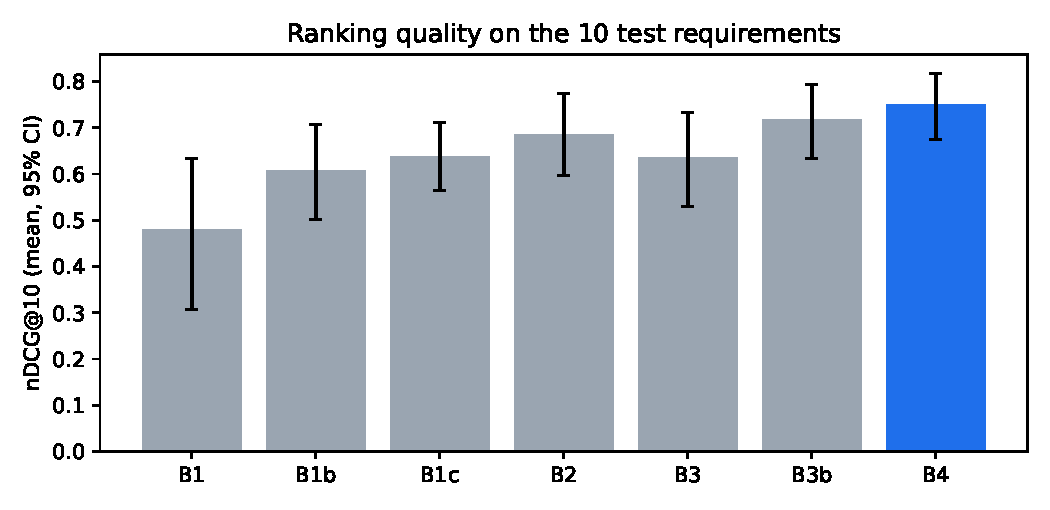
\includegraphics[width=\columnwidth]{figs/fig_ndcg10.pdf}
\caption{Mean nDCG@10 by method with 95\% bootstrap CIs over the \NTest{} test requirements; the proposed method (B4) is highlighted.}
\label{fig:ndcg}
\end{figure}

Table~\ref{tab:ats} shows how many qualified students each keyword rule rejects. The strict rule rejects \AtsStrictRejPct{}\% of them (\AtsStrictRejFail{} of \AtsStrictRejTotal{}), the lenient rule \AtsLenientRejPct{}\%, and the rule with synonyms \AtsSynRejPct{}\% (\AtsSynRejPctExact{}\% when only exact aliases match). The rate depends on how the resume is written. The strict rule rejects \AtsStrictRejStandardPct{}\% of qualified students with standard resumes, \AtsStrictRejImpliedPct{}\% of implied ones and \AtsStrictRejAbbreviatedNoisyPct{}\% of abbreviated, noisy ones. It rejects every paraphrased resume, but that is by construction, since those resumes contain no keywords. On average the strict rule leaves \AtsStrictPassMean{} students per requirement, between \AtsStrictPassMin{} and \AtsStrictPassMax{}.
\begin{table*}[!t]
\caption{Share of qualified students that each keyword rule rejects, pooled over the test requirements, by resume style; ``other'' pools generalist, ineligible-strong and stuffed resumes. Paraphrased resumes contain no keywords by construction.}
\label{tab:ats}
\centering\footnotesize
\resizebox{\textwidth}{!}{\begin{tabular}{lcccccccc}
\toprule
Method & Overall & standard & paraphrased & implied & abbrev.\ noisy & sparse strong & other (n) & Passers/req. \\
\midrule
B1 ATS strict & 56\% (106/190) & 22\% (17/77) & 100\% (51/51) & 56\% (10/18) & 86\% (18/21) & 36\% (4/11) & 50\% (6/12) & 0-20 (mean 10.5) \\
B1b ATS lenient (>=50\%) & 33\% (63/190) & 0\% (0/77) & 100\% (51/51) & 33\% (6/18) & 29\% (6/21) & 0\% (0/11) & 0\% (0/12) & 17-79 (mean 41.4) \\
B1c ATS + synonyms & 36\% (68/190) & 5\% (4/77) & 100\% (51/51) & 44\% (8/18) & 5\% (1/21) & 0\% (0/11) & 33\% (4/12) & 3-23 (mean 16.5) \\
\bottomrule
\end{tabular}
}
\end{table*}

Ranking quality is only part of the picture, because the re-ranker can only reorder the 20 resumes that retrieval returns. B4's pool holds \PoolPropTwenty{} of the \PoolQualifiedTotal{} qualified students, so its FRR@20 is \PropFrrtwentyCi{}. Hybrid ranking reaches \HybridFrrtwentyCi{} and ATS with synonyms \AtsSynFrrtwentyCi{}. B4 misses more than hybrid ranking on all ten requirements (difference \PropVsHybridFrrtwentyDiffCi{}). Fig.~\ref{fig:archetype} breaks the pools down by resume style. For implied resumes the dense pool finds \PoolDenseImpliedPct{}\% against \PoolAtsSynImpliedPct{}\% for the keyword rule with synonyms, but BM25 finds \PoolBmImpliedPct{}\%. For standard resumes the dense pool is the weakest method (\PoolDenseStandardPct{}\%). No method finds more than \PoolDenseParaphrasedPct{}\% of the paraphrased resumes. We therefore do not claim that PlaceIQ finds students a keyword filter misses in general; the evidence supports that only for implied skills, and only against keyword rules.
\begin{figure}[t]
\centering
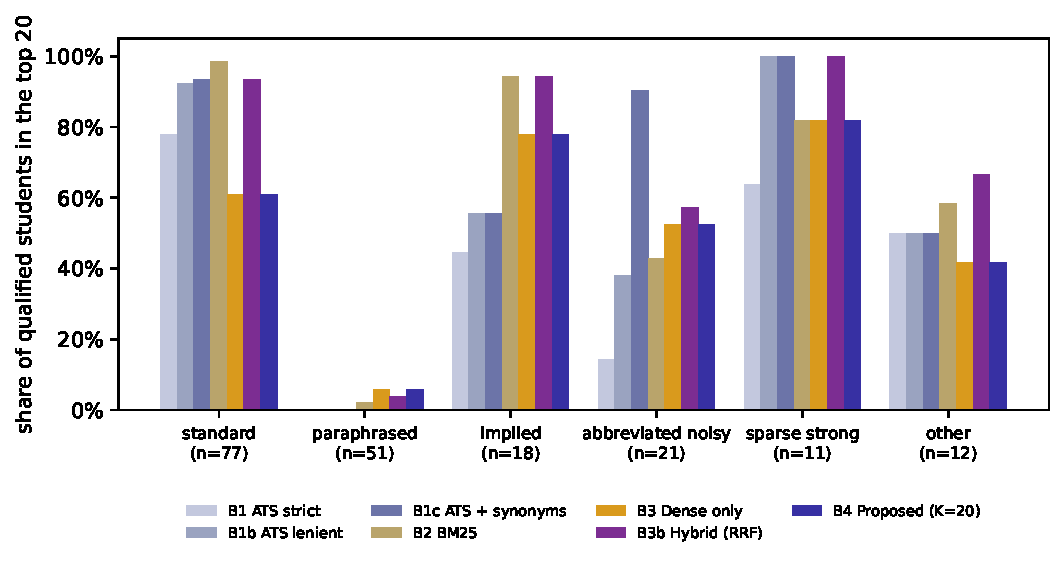
\includegraphics[width=\columnwidth]{figs/fig_archetype.pdf}
\caption{Share of qualified students inside each method's top-20 list, by resume style ($n$ is the number of qualified students in the group, pooled over the test requirements).}
\label{fig:archetype}
\end{figure}

The parser got all \ParserEligFieldsCorrect{} of \ParserEligFieldsTotal{} eligibility fields right on the development and test requirements (Table~\ref{tab:parser}), and no qualified student was lost to a parsed filter (\ParserFalseRej{} parser-caused false rejections). Skills are less clean. On the test requirements must-have precision is \ParserTestMustPrecPct{}\% and recall \ParserTestMustRecPct{}\%, with mismatches in \ParserTestMismatchReqs{} (test) and \ParserDevMismatchReqs{} (development), such as an extra keyword or a must-have demoted to nice-to-have. The requirements share the generator's style and 45 fields is a small sample, so this is not evidence about real postings.

Table~\ref{tab:ablations} lists the ablations. With $K=50$ the mean nDCG@10 is \PropKfiftyNdcgCi{} and FRR@20 falls from \PropFrrtwentyMean{} to \PropKfiftyFrrtwentyMean{}. Oracle filters and removing the fairness instruction change nDCG@10 by at most 0.006. None of the three nDCG differences is distinguishable from the main configuration.
\begin{table}[t]
\caption{Parser accuracy against the structured truth: exact match on the three eligibility fields, and precision and recall of the must-have skills after normalisation.}
\label{tab:parser}
\centering\scriptsize
\resizebox{\columnwidth}{!}{\begin{tabular}{lcccccc}
\toprule
Split & min\textbackslash{}\_cgpa & max\textbackslash{}\_backlogs & branches & Elig. & Must P & Must R \\
\midrule
dev & 100\% & 100\% & 100\% & 100\% & 100\% & 93\% \\
test & 100\% & 100\% & 100\% & 100\% & 96\% & 93\% \\
\bottomrule
\end{tabular}
}
\end{table}

\begin{table}[t]
\caption{Pre-declared ablations of the proposed method (K=50, oracle eligibility filters, no fairness instruction); means over the test requirements. None is distinguishable from the main configuration in nDCG@10. MRR is 1.000 for all variants except the fairness-off run (0.950); FRR@10 equals one minus capped Recall@10.}
\label{tab:ablations}
\centering\footnotesize
\begin{tabular}{lccc}
\toprule
Variant & nDCG@10 & Recall@10 (capped) & FRR@20 \\
\midrule
B4 main (K=20) & 0.749 & 0.760 & 0.501 \\
K=50 & 0.763 & 0.770 & 0.308 \\
Oracle filters & 0.755 & 0.770 & 0.495 \\
No fairness instr. & 0.755 & 0.760 & 0.495 \\
\bottomrule
\end{tabular}

\end{table}

\section{Post-hoc Analyses (exploratory)}
\label{sec:posthoc}
We added two analyses after seeing the test results. Neither was planned, the main results above are unchanged, and both should be read as exploratory.

\textbf{B5: hybrid retrieval with the same re-ranker.} B5 takes the top 20 of the fused BM25 and dense ranking as the pool and re-ranks it with the unchanged prompt. The pool holds \PoolBFiveTwenty{} of \PoolQualifiedTotal{} qualified students, against \PoolPropTwenty{} for B4, and FRR@20 is \BFiveTestFrrtwentyCi{} (Table~\ref{tab:b5paired}). The difference from B4 is \BFiveVsPropFrrtwentyDiffCi{}, lower on all ten requirements. This pool is the same one hybrid ranking uses, so the gain comes from retrieval and not from the language model. Against ATS with synonyms, coverage is not distinguishable (\BFiveVsAtsSynFrrtwentyDiffCi{}). B5 reaches nDCG@10 of \BFiveTestNdcgCi{}. The difference from B4 is not distinguishable (\BFiveVsPropNdcgDiffCi{}). Against hybrid ranking it is \BFiveVsHybridNdcgDiffCi{}, where the lower bound is exactly zero, so we call it marginal. The hybrid pool still contains only \PoolBFiveParaphrasedFound{} of the \ArchParaphrasedQualified{} qualified paraphrased students.

\textbf{D1: can the re-ranker judge paraphrased resumes?} To separate a retrieval failure from a re-ranking failure, we score paraphrased resumes with retrieval bypassed. For each test requirement the candidate set holds every eligible, qualified paraphrased student plus 15 eligible students who are not qualified, at least five of them keyword-stuffed. Paraphrased qualified students (\DOneNPositive{}) average \DOnePosScore{} points and the non-qualified ones (\DOneNNegative{}) average \DOneNegScore{}, or \DOneStuffedScore{} for the stuffed resumes. The AUC is \DOneAucCi{}, with per-requirement values from \DOneAucMin{} to \DOneAucMax{}. When the re-ranker sees these resumes it can separate them, so the paraphrase failure of the main pipeline comes from retrieval. Why retrieval misses them is untested. Two possibilities are the small embedding model and a query that names technologies while the resume describes the work. The caveats are real: the negatives are an easy contrast, and the paraphrases come from fixed templates, so the AUC is probably optimistic. The per-requirement values are in Table~\ref{tab:d1}.

\begin{table}[t]
\caption{Post-hoc exploratory: paired differences of B5 (hybrid retrieval plus the same re-ranker) against B4, B3b and B1c on the test requirements. W/L/T counts requirements where B5 is better: higher for nDCG and Recall, lower for FRR@20.}
\label{tab:b5paired}
\centering\scriptsize
\resizebox{\columnwidth}{!}{% POST-HOC EXPLORATORY (designed after seeing the test results). FRR rows: lower is better.
\begin{tabular}{llccc}
\toprule
Comparison & Metric & Mean diff [CI] & W/L/T (B5) & Verdict \\
\midrule
B5 vs B4 & nDCG@10 & 0.022 [-0.047, 0.094] & 5/5/0 & not distinguishable \\
B5 vs B4 & Recall@10$^{cap}$ & 0.100 [-0.000, 0.210] & 6/1/3 & not distinguishable \\
B5 vs B4 & FRR@20 & -0.187 [-0.242, -0.131] & 10/0/0 & better \\
B5 vs B3b & nDCG@10 & 0.053 [0.000, 0.107] & 6/2/2 & better \\
B5 vs B3b & Recall@10$^{cap}$ & 0.060 [0.020, 0.100] & 5/0/5 & better \\
B5 vs B3b & FRR@20 & 0.000 [0.000, 0.000] & 0/0/10 & not distinguishable \\
B5 vs B1c & nDCG@10 & 0.133 [0.073, 0.194] & 9/1/0 & better \\
B5 vs B1c & Recall@10$^{cap}$ & 0.130 [0.040, 0.220] & 7/1/2 & better \\
B5 vs B1c & FRR@20 & -0.024 [-0.123, 0.052] & 2/3/5 & not distinguishable \\
\bottomrule
\end{tabular}
}
\end{table}

\section{Fairness Test}
We changed only the name in the resume header and measured how much the re-ranker's score moved. The candidates are the top 10 of each test requirement (\FairOnPairs{} requirement-candidate pairs). Each pair got four swapped resumes: one control with a different name from the same group, and three cross-group swaps. We ran every swap with the fairness instruction on and off, and checked in code that only the header line differed.

If names mattered, cross-group swaps should move scores more than control swaps. They did not (Fig.~\ref{fig:fair}). With the instruction on, the mean absolute score change is \FairOnAbsScoreControlCi{} for control swaps and \FairOnAbsScoreCrossGroupCi{} for cross-group swaps (difference \FairOnAbsScoreDiffCi{}). With it off, the values are \FairOffAbsScoreControlCi{} and \FairOffAbsScoreCrossGroupCi{} (difference \FairOffAbsScoreDiffCi{}). All differences include zero. The embedding similarity changes by \FairOnAbsSimControlMean{} for control and \FairOnAbsSimCrossGroupMean{} for cross-group swaps, so names do not enter at retrieval either.

The more uncomfortable finding is the noise. A header-only change moved the score by 5 points or more in \FairShareFiveMinPct{} to \FairShareFiveMaxPct{}\% of swaps in every condition, and moved the candidate across the top-10 boundary in 3 to 7\% of swaps (Table~\ref{tab:fair} lists the other measures). The score is sensitive to any change in the prompt text. We also looked at signed changes per name group, 22 comparisons in all. Two exclude zero, both with the instruction on: Gujarati female names (\FairOnSignedGujaratiFemaleCi{}) and the Gujarati group that contains them (\FairOnSignedRegionGujaratiCi{}). With this many comparisons that may be chance, and the same names show no shift with the instruction off. We therefore report that no name effect was detected, not that the system is unbiased. The test covers names only, not college prestige or other proxies.

\begin{figure}[t]
\centering
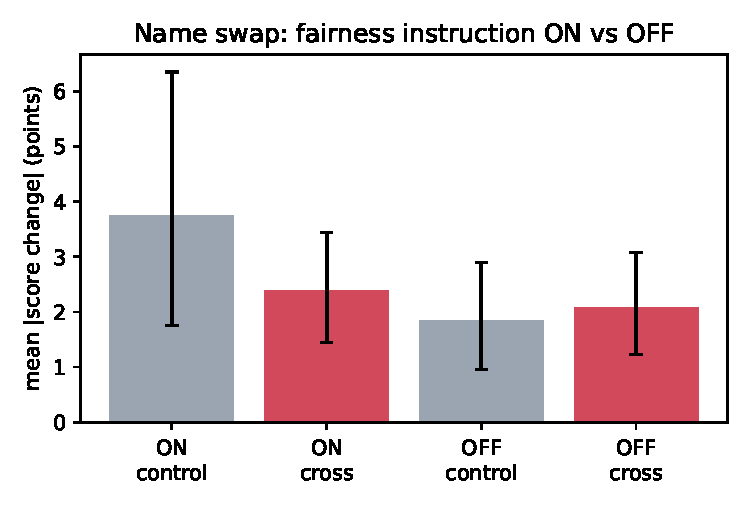
\includegraphics[width=0.85\columnwidth]{figs/fig_fairness.pdf}
\caption{Mean absolute score change after replacing the name in the resume header: a same-group name (control) versus names from other groups, with the fairness instruction on and off; 95\% bootstrap CIs over \FairOnPairs{} requirement-candidate pairs. Names only.}
\label{fig:fair}
\end{figure}

\FloatBarrier
\section{Prototype Extensions}\label{sec:ext}
After the demonstration we added two features to the demo application. One lists all suited candidates beside the top 10. The other shows a student where they fall short for a given company. We did not evaluate either one. The results in the earlier sections cover only the frozen top-10 pipeline.

\textbf{Full suited list.} The new mode retrieves with the hybrid ranking (BM25 and dense scores fused by reciprocal rank fusion, $k=60$), takes the 50 best candidates and scores all of them with the same re-ranker. The first ten are labelled Top 10. The rest are labelled Also suited if their score is at least 60 and below threshold otherwise. The application reports how many students are suited out of how many are eligible, and offers the list as a CSV file. Because this pool comes from hybrid retrieval, its top 10 can differ from the top 10 of the main pipeline, which uses a dense pool. For one benchmark requirement (R02), 319 students were eligible and 43 reached the threshold. For a data-engineer requirement we wrote ourselves, 247 were eligible and 34 reached it. Scoring 50 candidates took 146\,s cold on the 6\,GB laptop, about 2.4\,s each. Students outside the pool are never scored, so the list keeps the coverage limit described in Section~\ref{sec:posthoc}.

\textbf{Student view.} For one student and one requirement, the view shows the score with the matched and missing skills, and a table that checks CGPA, branch and backlogs against the rules (these are marked as not fixable by editing the resume). Each missing skill gets a suggestion card with a reason, a small project that extends the student's own work, learning steps, and a sample resume bullet to use only after the work is done. The suggestion prompt never sees the resume header. A validator rejects placeholders, links, numbers and outcome claims in the sample bullet, and a skill that fails twice shows a message instead of a suggestion; two of the seven suggestions in our check failed this way.

\textbf{What-if.} The main what-if is arithmetic: if the student gains the ticked skills, how many required and nice-to-have skills would be matched. It is not a predicted score or rank. A second option writes one sample project bullet per ticked skill, appends it to a copy of the resume, and re-scores the copy with the same re-ranker. It also embeds the changed text in memory and recomputes the hybrid rank, without writing to the vector index. Table~\ref{tab:whatif} lists what happened for four students.

\begin{table}[!t]
\caption{What-if re-scoring for four students (examples, not measurements). The first two rows use an earlier version that appended a hypothetical bullet or an assumed-skills line for one skill (TypeScript).}
\label{tab:whatif}
\centering\scriptsize
\resizebox{\columnwidth}{!}{%
\begin{tabular}{llcc}
\toprule
Student & Change & Score & Hybrid rank\\
\midrule
S216, R02 & Hypothetical bullet (earlier version) & 85 $\to$ 40 & --\\
S216, R02 & Assumed-skills line (earlier version) & 85 $\to$ 60 & --\\
S253, R02 & Three sample bullets & 60 $\to$ 100 & 10 $\to$ 2\\
S078, data engineer & One sample bullet (Airflow) & 65 $\to$ 100 & 11 $\to$ 7\\
S243, R02 & No bullet passed validation & 65 $\to$ 65 & 38 $\to$ 38\\
\bottomrule
\end{tabular}}
\end{table}

The results do not agree with each other. The earlier version lowered a score, while the later one raised two scores to 100. For S078 the re-ranker credited ETL Pipelines although only an Airflow bullet had been added. The hybrid rank moved mostly through BM25, because the added bullets contain the missing keywords, and dense similarity moved by at most 0.020. So the re-score only shows how a small model reacts to added text. The same property makes it easy to game, so we do not present it as a prediction. We also found two candidates in the data-engineer list that scored 100 while the re-ranker listed a required skill as missing, although its prompt caps such a score at 69. The full list does not enforce that cap. The coverage line and the suggestions are therefore the main output of the student view.

\section{Discussion and Limitations}
\textbf{What the evidence supports.} On this benchmark, LLM re-ranking improves the top of the list over dense retrieval and over the keyword rules, and it puts a qualified student first for every test requirement. Keyword rejection depends strongly on how a resume is written, and it stays high even when synonyms are matched. The main weakness is coverage. The re-ranker sees only what retrieval returns, a hybrid pool recovers many more qualified students than a dense one, and the paraphrased resumes are lost before the re-ranker sees them. Re-ranking by itself did not beat a hybrid ranking of BM25 and dense scores, which needs no language model.

\textbf{Limitations.} Everything here is synthetic, and the labels come from the same generator as the resumes, so the results show differences between methods and say nothing about real placement outcomes. The spot check had one labeller and 20 pairs. The paraphrases come from a fixed set of 6 to 10 sentences per skill, which probably makes retrieval look better than it would on real resumes. The test has ten requirements, so the intervals are wide and a single requirement can move a mean. We simplified some requirements and edited the taxonomy during balancing, and B1c borrows aliases from the generator. The re-ranker prompt was revised once on the development set, one code change followed the freeze, and B5 and D1 were designed after the test results. MRR is computed on lists cut at 20. The parser was tested on requirements written in the generator's own style. The fairness test covers names only. The prototype extensions are shown on a handful of examples and were not evaluated. PlaceIQ is meant as decision support: a person should read every shortlist.

\textbf{Future work.} The first need is real resumes with labels from placement officers. On the method side, retrieval for paraphrased resumes needs work, for example a larger embedding model, several queries per requirement, or indexing extracted skills and projects separately. Both are untested ideas here, as are the five ideas in Table~\ref{tab:random}. Fairness testing should also cover college names and other proxies.

\section{Conclusion}
We built PlaceIQ, a local pipeline that parses a free-text requirement, filters by eligibility, retrieves resumes and re-ranks them with explanations, and we compared it with keyword filters and retrieval baselines on a synthetic benchmark of \NStudents{} students. LLM re-ranking improved ranking quality over dense retrieval and keyword rules, keyword filters rejected a large share of qualified students, and no name effect was detected. We also describe two unevaluated extensions, a list of all suited candidates and feedback for students. Retrieval coverage limited the pipeline, and it did not beat hybrid search. Real resumes, human labels and better retrieval for paraphrased text are the next steps. The code, evaluation scripts and demo application are public at \url{https://github.com/24Chessman/PlaceIQ}.

\appendices
\section{Additional Tables}
These tables hold detail that the main text summarises with the numbers in \texttt{numbers.tex}. The B5 tables are post-hoc exploratory: B5 and D1 were designed after the test results were known.

\begin{table*}[!tb]
\caption{Share of qualified students inside the top-20 pool, by resume style (counts in brackets), pooled over the test requirements.}
\label{tab:archetype}
\centering\small
\resizebox{\textwidth}{!}{\begin{tabular}{lcccccccc}
\toprule
Method & standard & paraphrased & implied & abbreviated\_noisy & sparse\_strong & ineligible\_strong & generalist\_average & stuffed\_weak \\
\midrule
B1 ATS strict & 78\% (60/77) & 0\% (0/51) & 44\% (8/18) & 14\% (3/21) & 64\% (7/11) & 100\% (1/1) & 62\% (5/8) & 0\% (0/3) \\
B1b ATS lenient (>=50\%) & 92\% (71/77) & 0\% (0/51) & 56\% (10/18) & 38\% (8/21) & 100\% (11/11) & 100\% (1/1) & 38\% (3/8) & 67\% (2/3) \\
B1c ATS + synonyms & 94\% (72/77) & 0\% (0/51) & 56\% (10/18) & 90\% (19/21) & 100\% (11/11) & 100\% (1/1) & 62\% (5/8) & 0\% (0/3) \\
B2 BM25 & 99\% (76/77) & 2\% (1/51) & 94\% (17/18) & 43\% (9/21) & 82\% (9/11) & 100\% (1/1) & 75\% (6/8) & 0\% (0/3) \\
B3 Dense only & 61\% (47/77) & 6\% (3/51) & 78\% (14/18) & 52\% (11/21) & 82\% (9/11) & 100\% (1/1) & 50\% (4/8) & 0\% (0/3) \\
B3b Hybrid (RRF) & 94\% (72/77) & 4\% (2/51) & 94\% (17/18) & 57\% (12/21) & 100\% (11/11) & 100\% (1/1) & 88\% (7/8) & 0\% (0/3) \\
B4 Proposed (K=20) & 61\% (47/77) & 6\% (3/51) & 78\% (14/18) & 52\% (11/21) & 82\% (9/11) & 100\% (1/1) & 50\% (4/8) & 0\% (0/3) \\
\bottomrule
\end{tabular}
}
\end{table*}

\begin{table*}[!tb]
\caption{Post-hoc exploratory: B5 (hybrid retrieval plus the same re-ranker), mean with 95\% bootstrap CI over requirements (dev and test shown separately).}
\label{tab:b5}
\centering\small
\resizebox{\textwidth}{!}{% POST-HOC EXPLORATORY (designed after seeing the test results)
\begin{tabular}{lcccccc}
\toprule
Method (post-hoc) & nDCG@10 & MRR & P@10 & Recall@10 (capped) & FRR@10 & FRR@20 \\
\midrule
B5 hybrid + LLM re-rank, dev (n=5) & 0.724 [0.574, 0.838] & 1.000 [1.000, 1.000] & 0.740 [0.540, 0.920] & 0.740 [0.540, 0.920] & 0.260 [0.080, 0.460] & 0.393 [0.290, 0.477] \\
B5 hybrid + LLM re-rank, test (n=10) & 0.772 [0.707, 0.824] & 1.000 [1.000, 1.000] & 0.860 [0.790, 0.930] & 0.860 [0.790, 0.930] & 0.140 [0.070, 0.210] & 0.314 [0.233, 0.384] \\
\bottomrule
\end{tabular}
}
\end{table*}

\begin{table*}[!tb]
\caption{Post-hoc exploratory: share of qualified students inside the candidate pool, for the dense pool (B4), the hybrid ranking (B3b) and the hybrid pool (B5).}
\label{tab:b5arch}
\centering\small
\resizebox{\textwidth}{!}{% POST-HOC EXPLORATORY (designed after seeing the test results)
\begin{tabular}{lcccccccc}
\toprule
Pool (post-hoc) & standard & paraphrased & implied & abbreviated\_noisy & sparse\_strong & ineligible\_strong & generalist\_average & stuffed\_weak \\
\midrule
B4 (dense pool) & 61\% (47/77) & 6\% (3/51) & 78\% (14/18) & 52\% (11/21) & 82\% (9/11) & 100\% (1/1) & 50\% (4/8) & 0\% (0/3) \\
B3b hybrid ranking (no LLM) & 94\% (72/77) & 4\% (2/51) & 94\% (17/18) & 57\% (12/21) & 100\% (11/11) & 100\% (1/1) & 88\% (7/8) & 0\% (0/3) \\
B5 (hybrid pool) & 94\% (72/77) & 4\% (2/51) & 94\% (17/18) & 57\% (12/21) & 100\% (11/11) & 100\% (1/1) & 88\% (7/8) & 0\% (0/3) \\
\bottomrule
\end{tabular}
}
\end{table*}

\begin{table*}[!tb]
\caption{Name-swap test: control (same-group name) versus cross-group names, with the fairness instruction on and off.}
\label{tab:fair}
\centering\small
\resizebox{\textwidth}{!}{\begin{tabular}{llccc}
\toprule
Condition & Metric & Control & Cross-group & Cross$-$control \\
\midrule
instruction ON & mean abs score change (points) & 3.750 [1.750, 6.350] & 2.383 [1.450, 3.433] & -1.367 [-3.517, 0.250] (not distinguishable) \\
instruction ON & share of swaps with abs change >= 5 & 0.170 [0.100, 0.250] & 0.160 [0.103, 0.223] & -0.010 [-0.073, 0.053] (not distinguishable) \\
instruction ON & mean abs rank shift in 20-pool & 0.710 [0.330, 1.140] & 0.403 [0.220, 0.617] & -0.307 [-0.697, 0.047] (not distinguishable) \\
instruction ON & top-10 boundary-crossing rate & 0.070 [0.020, 0.120] & 0.033 [0.013, 0.060] & -0.037 [-0.083, 0.007] (not distinguishable) \\
instruction ON & mean abs cosine-similarity shift (retrieval) & 0.014 [0.012, 0.016] & 0.014 [0.013, 0.015] & -0.000 [-0.002, 0.002] (not distinguishable) \\
instruction OFF & mean abs score change (points) & 1.850 [0.950, 2.900] & 2.083 [1.233, 3.083] & 0.233 [-0.617, 1.100] (not distinguishable) \\
instruction OFF & share of swaps with abs change >= 5 & 0.150 [0.080, 0.220] & 0.143 [0.090, 0.203] & -0.007 [-0.060, 0.043] (not distinguishable) \\
instruction OFF & mean abs rank shift in 20-pool & 0.580 [0.250, 0.980] & 0.577 [0.283, 0.940] & -0.003 [-0.263, 0.240] (not distinguishable) \\
instruction OFF & top-10 boundary-crossing rate & 0.060 [0.020, 0.110] & 0.063 [0.027, 0.107] & 0.003 [-0.023, 0.030] (not distinguishable) \\
instruction OFF & mean abs cosine-similarity shift (retrieval) & 0.014 [0.012, 0.016] & 0.014 [0.013, 0.015] & -0.000 [-0.002, 0.002] (not distinguishable) \\
\bottomrule
\end{tabular}
}
\end{table*}
\begin{table}[!t]
\caption{Post-hoc exploratory: D1, scoring paraphrased resumes with retrieval bypassed (per requirement).}
\label{tab:d1}
\centering\scriptsize
\resizebox{\columnwidth}{!}{% POST-HOC EXPLORATORY (designed after seeing the test results)
\begin{tabular}{lcccccc}
\toprule
Req & Para. qual. & Non-qual. & Score qual. & Score non-qual. & AUC & Top-10 \\
\midrule
R02 & 4 & 15 & 83.8 & 42.4 & 0.808 & 4/4 \\
R03 & 5 & 15 & 62.0 & 17.1 & 0.947 & 5/5 \\
R05 & 6 & 15 & 95.0 & 32.9 & 0.867 & 6/6 \\
R06 & 3 & 15 & 85.0 & 47.7 & 0.844 & 3/3 \\
R08 & 7 & 15 & 94.3 & 16.7 & 0.995 & 7/7 \\
R10 & 6 & 15 & 83.3 & 35.1 & 0.900 & 6/6 \\
R11 & 3 & 15 & 86.7 & 22.3 & 0.956 & 3/3 \\
R13 & 7 & 15 & 49.3 & 25.7 & 0.767 & 6/7 \\
R14 & 5 & 15 & 100.0 & 32.7 & 0.933 & 5/5 \\
R15 & 5 & 15 & 81.8 & 22.2 & 0.847 & 4/5 \\
\bottomrule
\end{tabular}
}
\end{table}

\FloatBarrier


\bibliographystyle{IEEEtran}
\bibliography{refs}
\end{document}
